% Created 2021-05-24 Mon 10:45
% Intended LaTeX compiler: pdflatex
\documentclass[presentation]{beamer}
\usepackage[utf8]{inputenc}
\usepackage[T1]{fontenc}
\usepackage{graphicx}
\usepackage{grffile}
\usepackage{longtable}
\usepackage{wrapfig}
\usepackage{rotating}
\usepackage[normalem]{ulem}
\usepackage{amsmath}
\usepackage{textcomp}
\usepackage{amssymb}
\usepackage{capt-of}
\usepackage{hyperref}
\usetheme{Madrid}
\author{Daniel Coral\thanks{daniel.coral@med.lu.se}}
\date{\today}
\title{Discordant variant analysis}
\institute{GAME unit}
\hypersetup{
 pdfauthor={Daniel Coral},
 pdftitle={Discordant variant analysis},
 pdfkeywords={},
 pdfsubject={},
 pdfcreator={Emacs 27.1 (Org mode 9.3)}, 
 pdflang={English}}
\begin{document}

\maketitle
\begin{frame}{Outline}
\tableofcontents
\end{frame}


\begin{frame}[label={sec:org6888ea1}]{Background}
\begin{itemize}
\item The relationship between obesity and cardiometabolic risk is highly heterogeneous.
\item Individuals in the same BMI level may display different cardiometabolic risk:
\begin{itemize}
\item \textasciitilde{} 30\% of people with a BMI > 30 kg/m\textsuperscript{2} display a protective metabolic profile.
\item \textasciitilde{} 30\% of people with BMI < 25 kg/m\textsuperscript{2} develop conditions usually associated with obesity.
\end{itemize}
\item Better risk stratification and more precise interventions may improve outcomes.
\item Obesity and T2D are closely linked.
\item T2D is in turn, linked to many cardiovascular diseases, and is life-threatening.
\item Factors uncoupling obesity from T2D risk may be used to define clinically relevant subgroups of obesity.
\end{itemize}
\end{frame}
\begin{frame}[label={sec:orge7b7d87}]{Aims}
\begin{itemize}
\item Use genetics to stratify obesity into 2 subtypes:
\begin{itemize}
\item Concordant (\(\uparrow\) BMI and \(\uparrow\) T2D)
\item Discordant (\(\uparrow\) BMI and \(\downarrow\) T2D).
\end{itemize}
\item Perform a phenome-wide scan to detect traits that reinforce this stratification.
\item Leverage this information for further stratification with potential clinical meaning.
\end{itemize}
\end{frame}
\begin{frame}[label={sec:org37950cb}]{Analysis pipeline}
\begin{figure}[htbp]
\centering
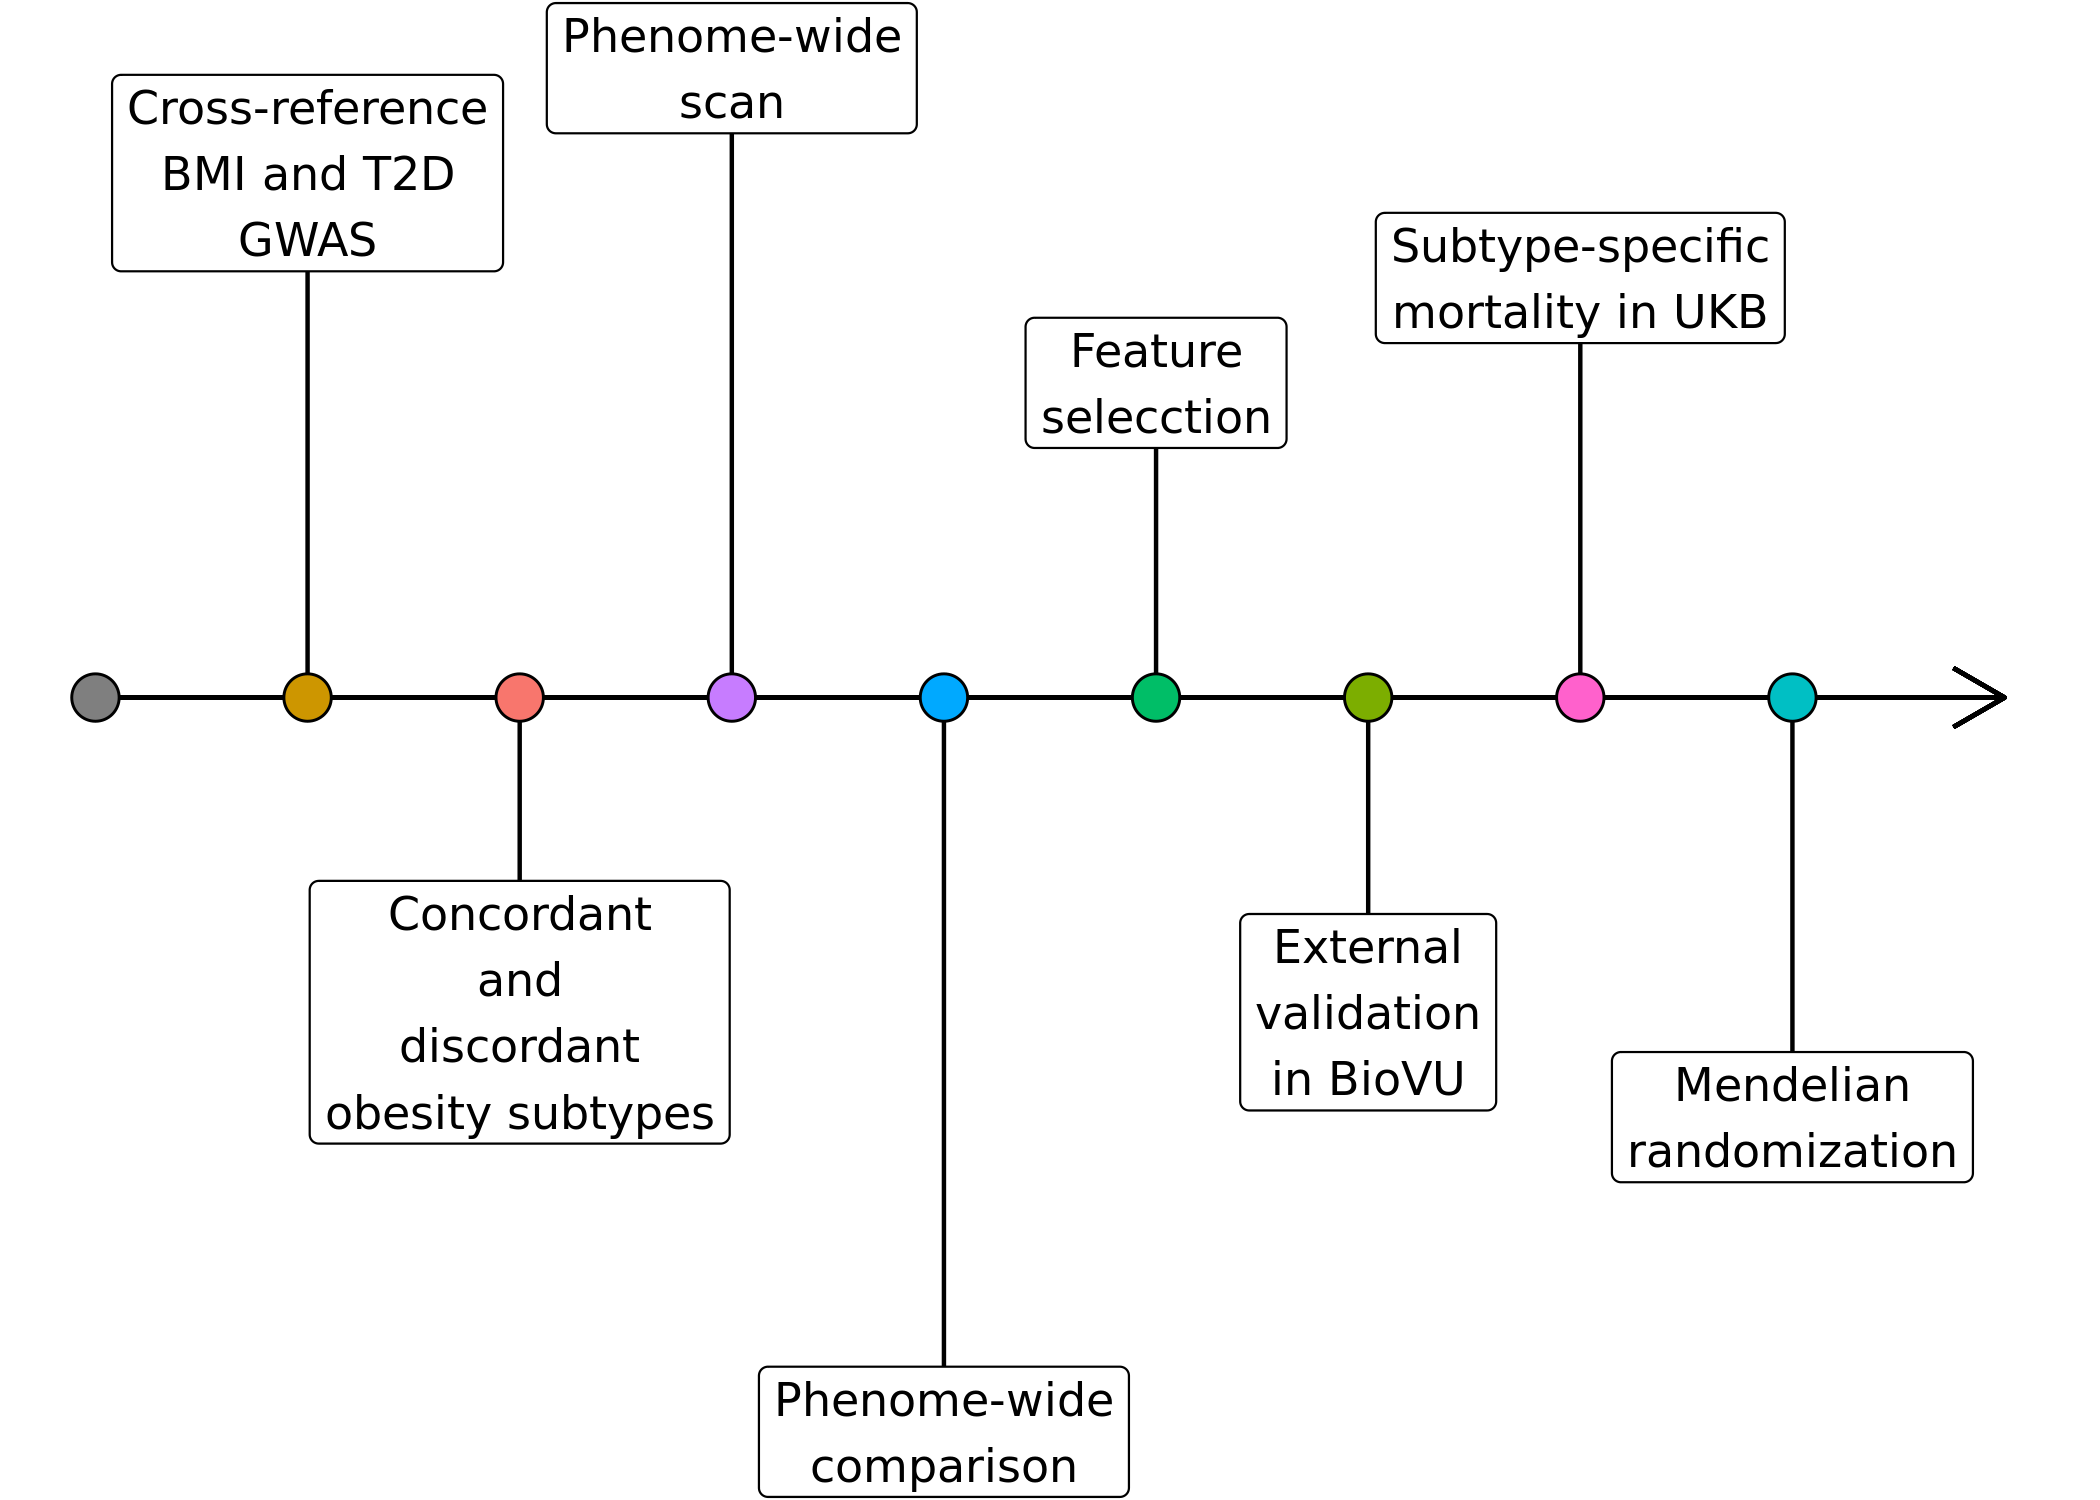
\includegraphics[width=.9\linewidth]{./plots/aline_plot.png}
\caption{Analysis flowchart}
\end{figure}
\end{frame}
\begin{frame}[label={sec:org9d4be89}]{BMI and T2D GWAS}
\begin{itemize}
\item BMI: Yengo \emph{et al.} (2018) vs T2D: Mahajan \emph{et al} (2018).
\begin{itemize}
\item Common biallelic variants (MAF > 1\%)
\item No INDELs
\item No potentially ambiguous palindromic SNPs (MAF > 30\%)
\item More than 20 \% difference in MAF with 1000G EUR
\item Clumpling (\emph{r\textsuperscript{2}} < 0.01 over 500kb window in 1000G EUR)
\end{itemize}
\end{itemize}
\end{frame}
\begin{frame}[label={sec:org40ae64d}]{Cross-referencing}
\begin{center}
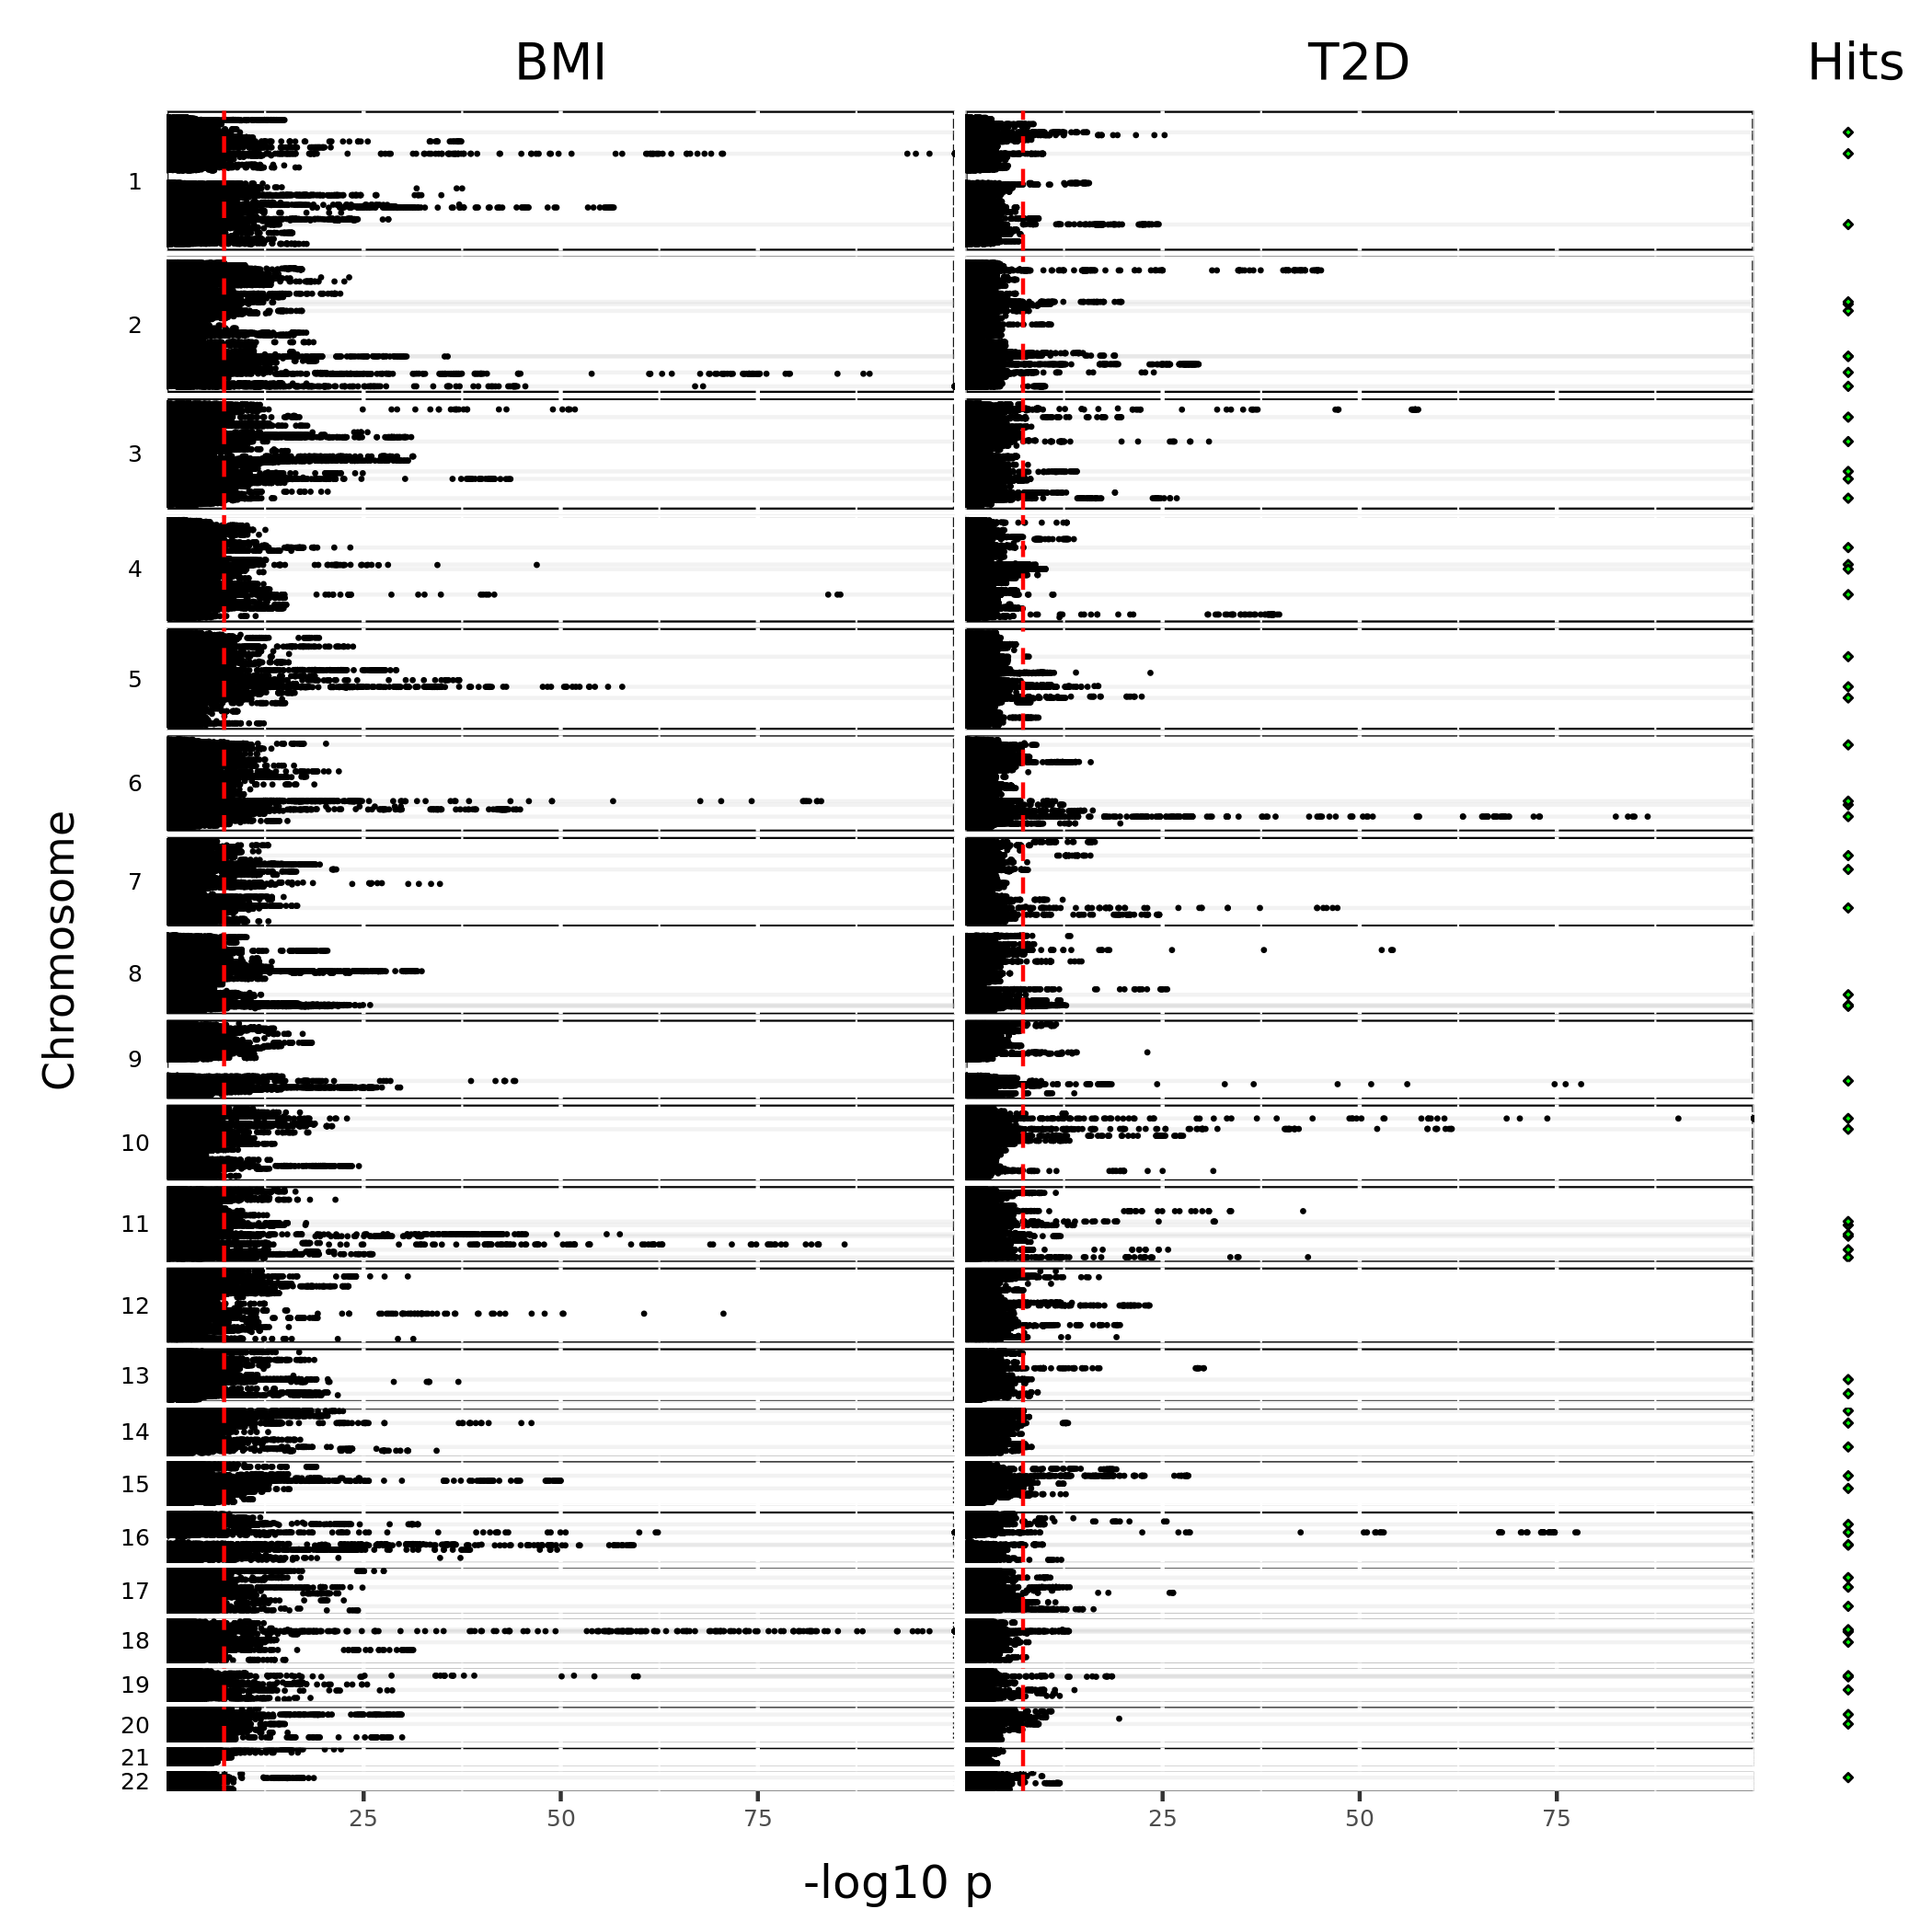
\includegraphics[width=7cm]{./plots/gmirror.png}
\end{center}
\end{frame}
\begin{frame}[label={sec:org55b8148}]{Assembly of concordant and discordant profiles}
\begin{figure}[htbp]
\centering
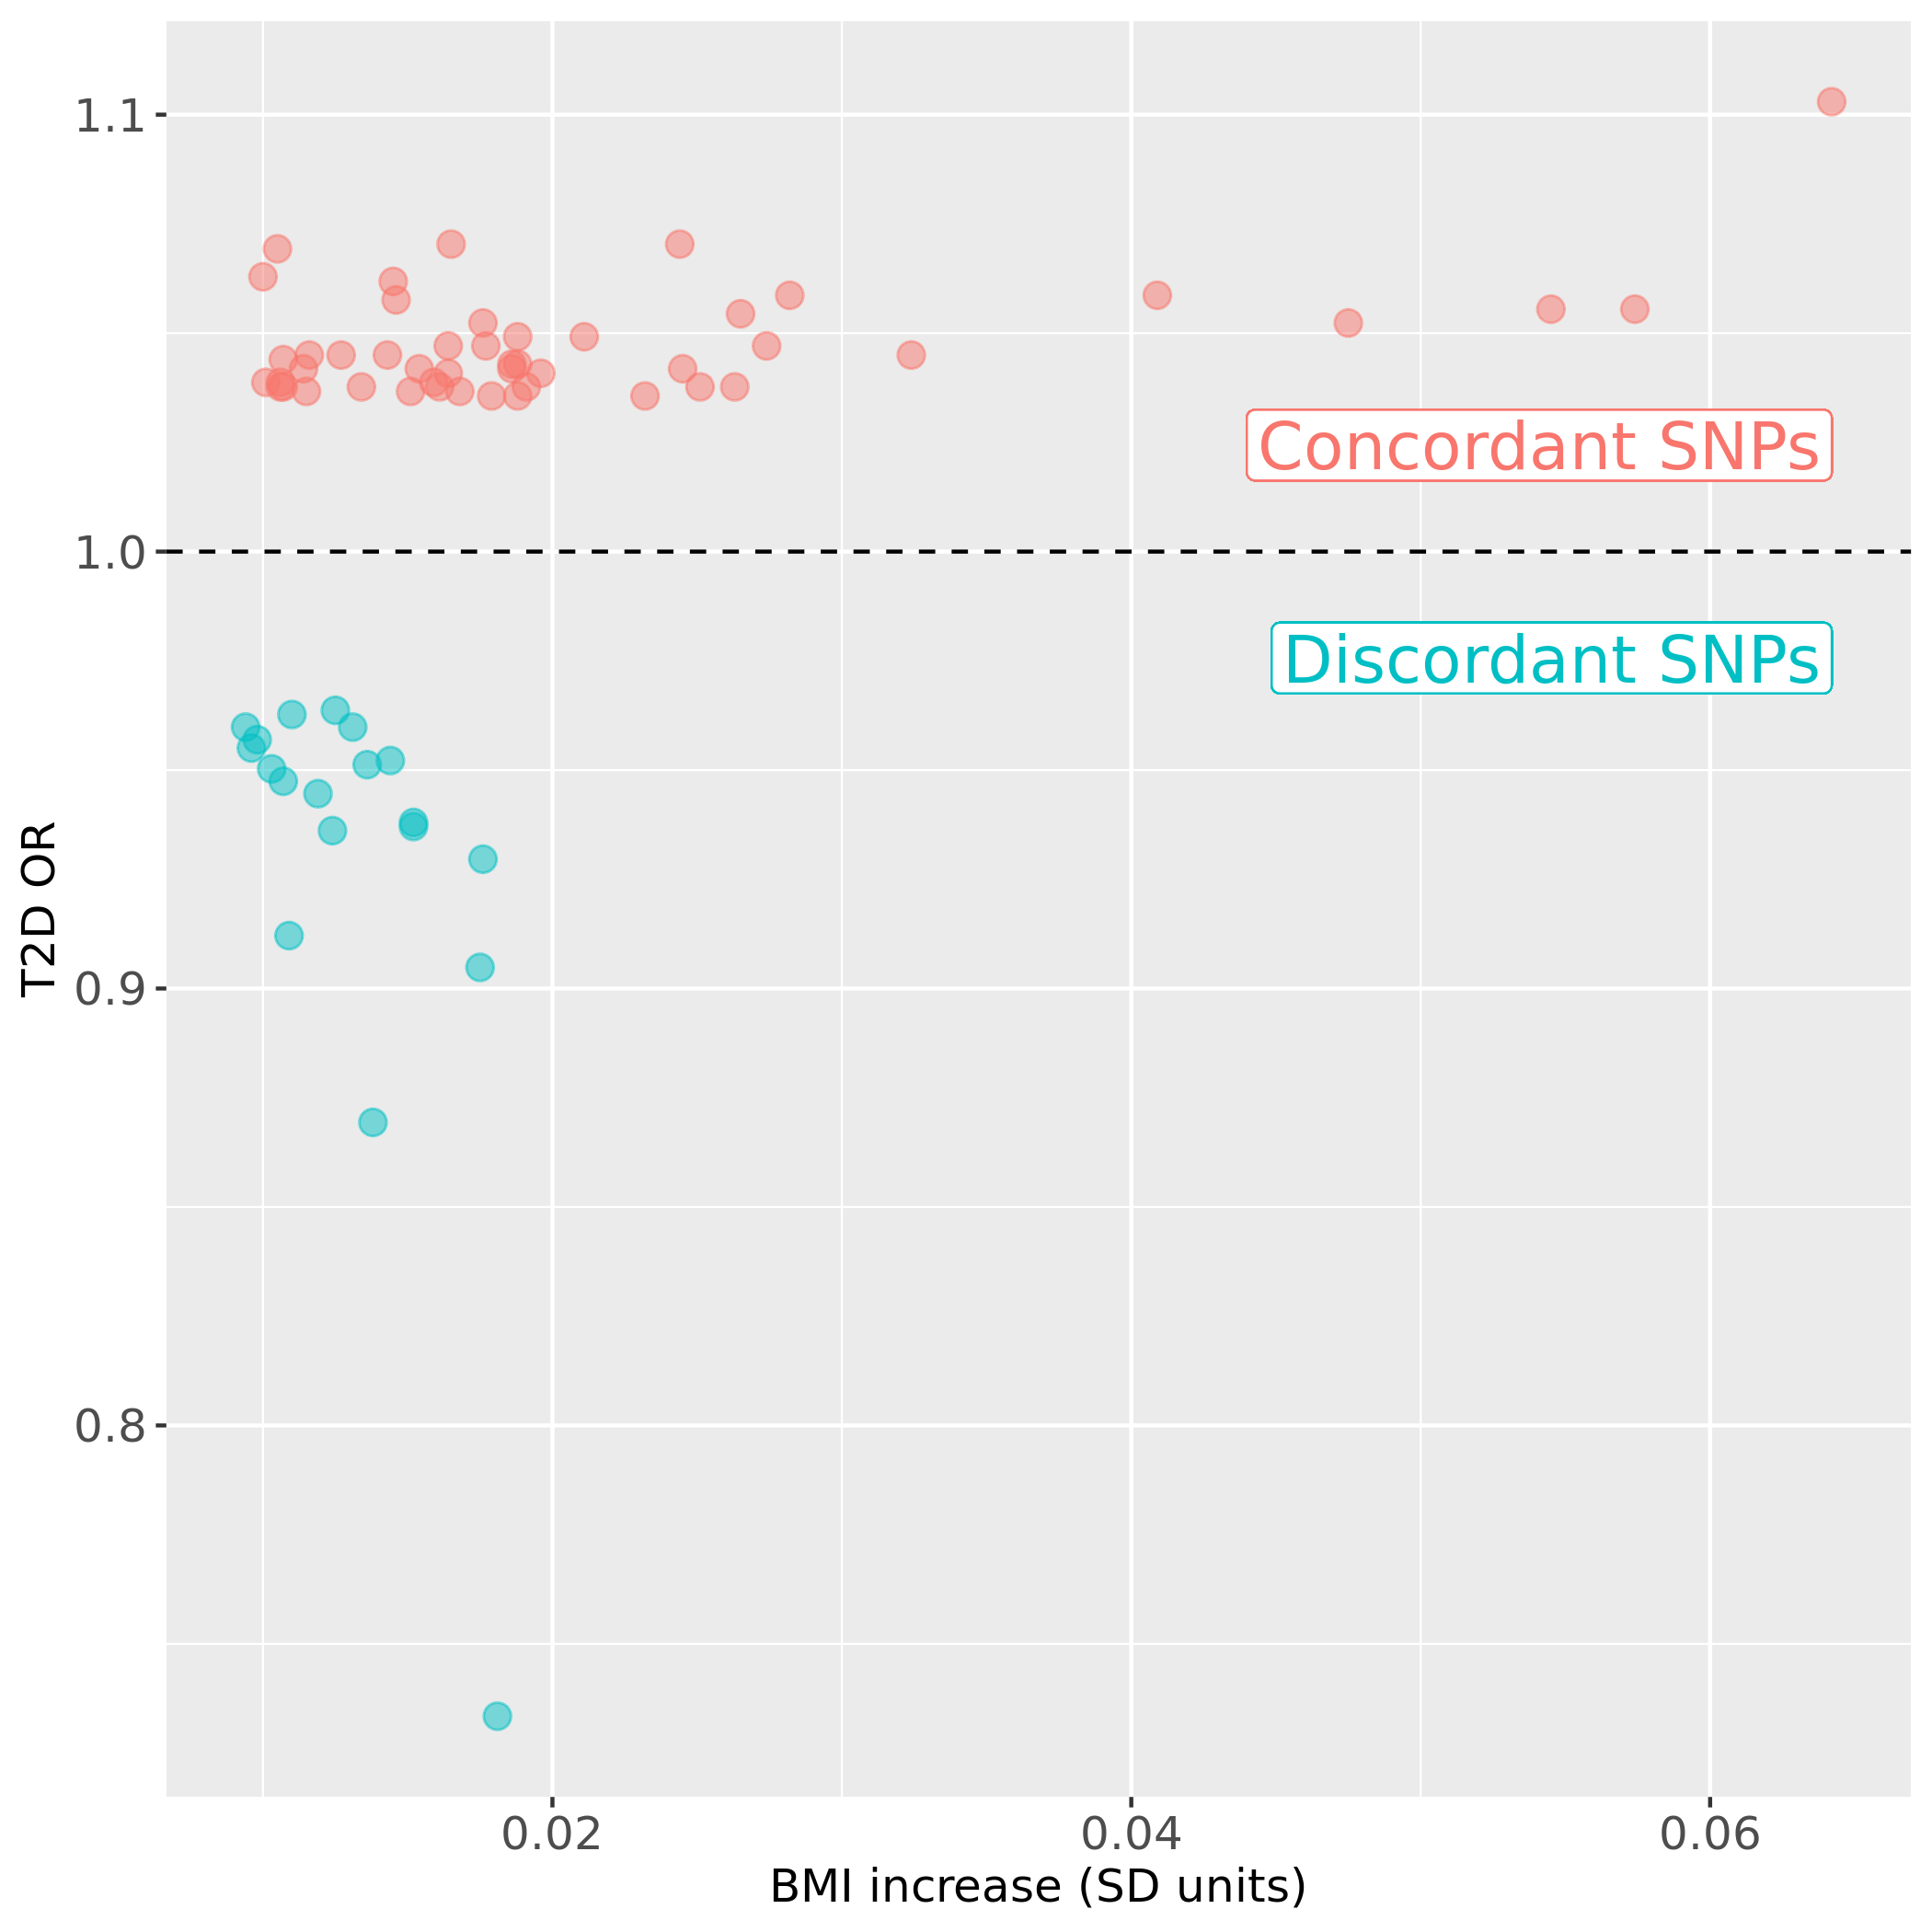
\includegraphics[width=6cm]{./plots/profiles.png}
\caption{Lead variants aligned to the BMI increasing allele and stratified by their \(\beta\) coefficient for T2D.}
\end{figure}
\end{frame}
\begin{frame}[label={sec:orgb6561a1}]{Phenome-wide scan - Data collection}
\begin{itemize}
\item MRC IEU GWAS database
\item Associations of lead SNPs or nearest proxy if missing 
\begin{itemize}
\item \emph{r\textsuperscript{2}} < 0.01 over 500kb window in 1000G EUR
\end{itemize}
\item Studies in EUR
\item More than 500 individuals
\item More than 25 minor alleles in smallest group for binary traits
\item Studies with information for all reference SNPs
\item If multiple studies for a single trait:
\begin{itemize}
\item The study with the highest sample size was selected
\end{itemize}
\item \textasciitilde{} 3500 traits
\end{itemize}
\end{frame}
\begin{frame}[label={sec:org7a266a2}]{Phenome-wide comparison}
\begin{itemize}
\item Two-stage analysis
\begin{itemize}
\item Univariate comparison - Random effects meta-analysis
\item Clustering and selection of traits - Random forest
\end{itemize}
\end{itemize}
\end{frame}
\begin{frame}[label={sec:org0fd4548}]{Phenome-wide comparison - Univariate analysis}
\begin{itemize}
\item Pooled concordant (\(\beta_C\)) and discordant (\(\beta_D\)) effects for each trait
\begin{enumerate}
\item Standardized beta coefficients: ~ \(SE = 1/\sqrt{2 * MAF * (1 - MAF) * (n + Z^2)}\)
\item Random effects meta-analysis (Paule-Mandel \(\tau\) estimator)
\end{enumerate}
\item Difference between pooled estimates (\emph{D})
\end{itemize}
\begin{align*}
D & = |\beta_C - \beta_D|\\
\\
SE_D & = \sqrt{{SE_C}^2 + {SE_D}^2}\\
\\
Z & = \frac{D}{SE_D} \sim \mathcal{N}(0,\,{SE_D}^{2})
\end{align*}
\begin{itemize}
\item Selection of traits: ( ~ \(\beta_C \ne 0\) ~ | ~ \(\beta_D \ne 0\) ~ ) ~ \& ~ \(D \ne 0\)
\begin{itemize}
\item FDR 10\%
\end{itemize}
\item 195 traits
\end{itemize}
\end{frame}
\begin{frame}[label={sec:orgfc05592}]{Results of univariate comparison}
\begin{figure}[htbp]
\centering
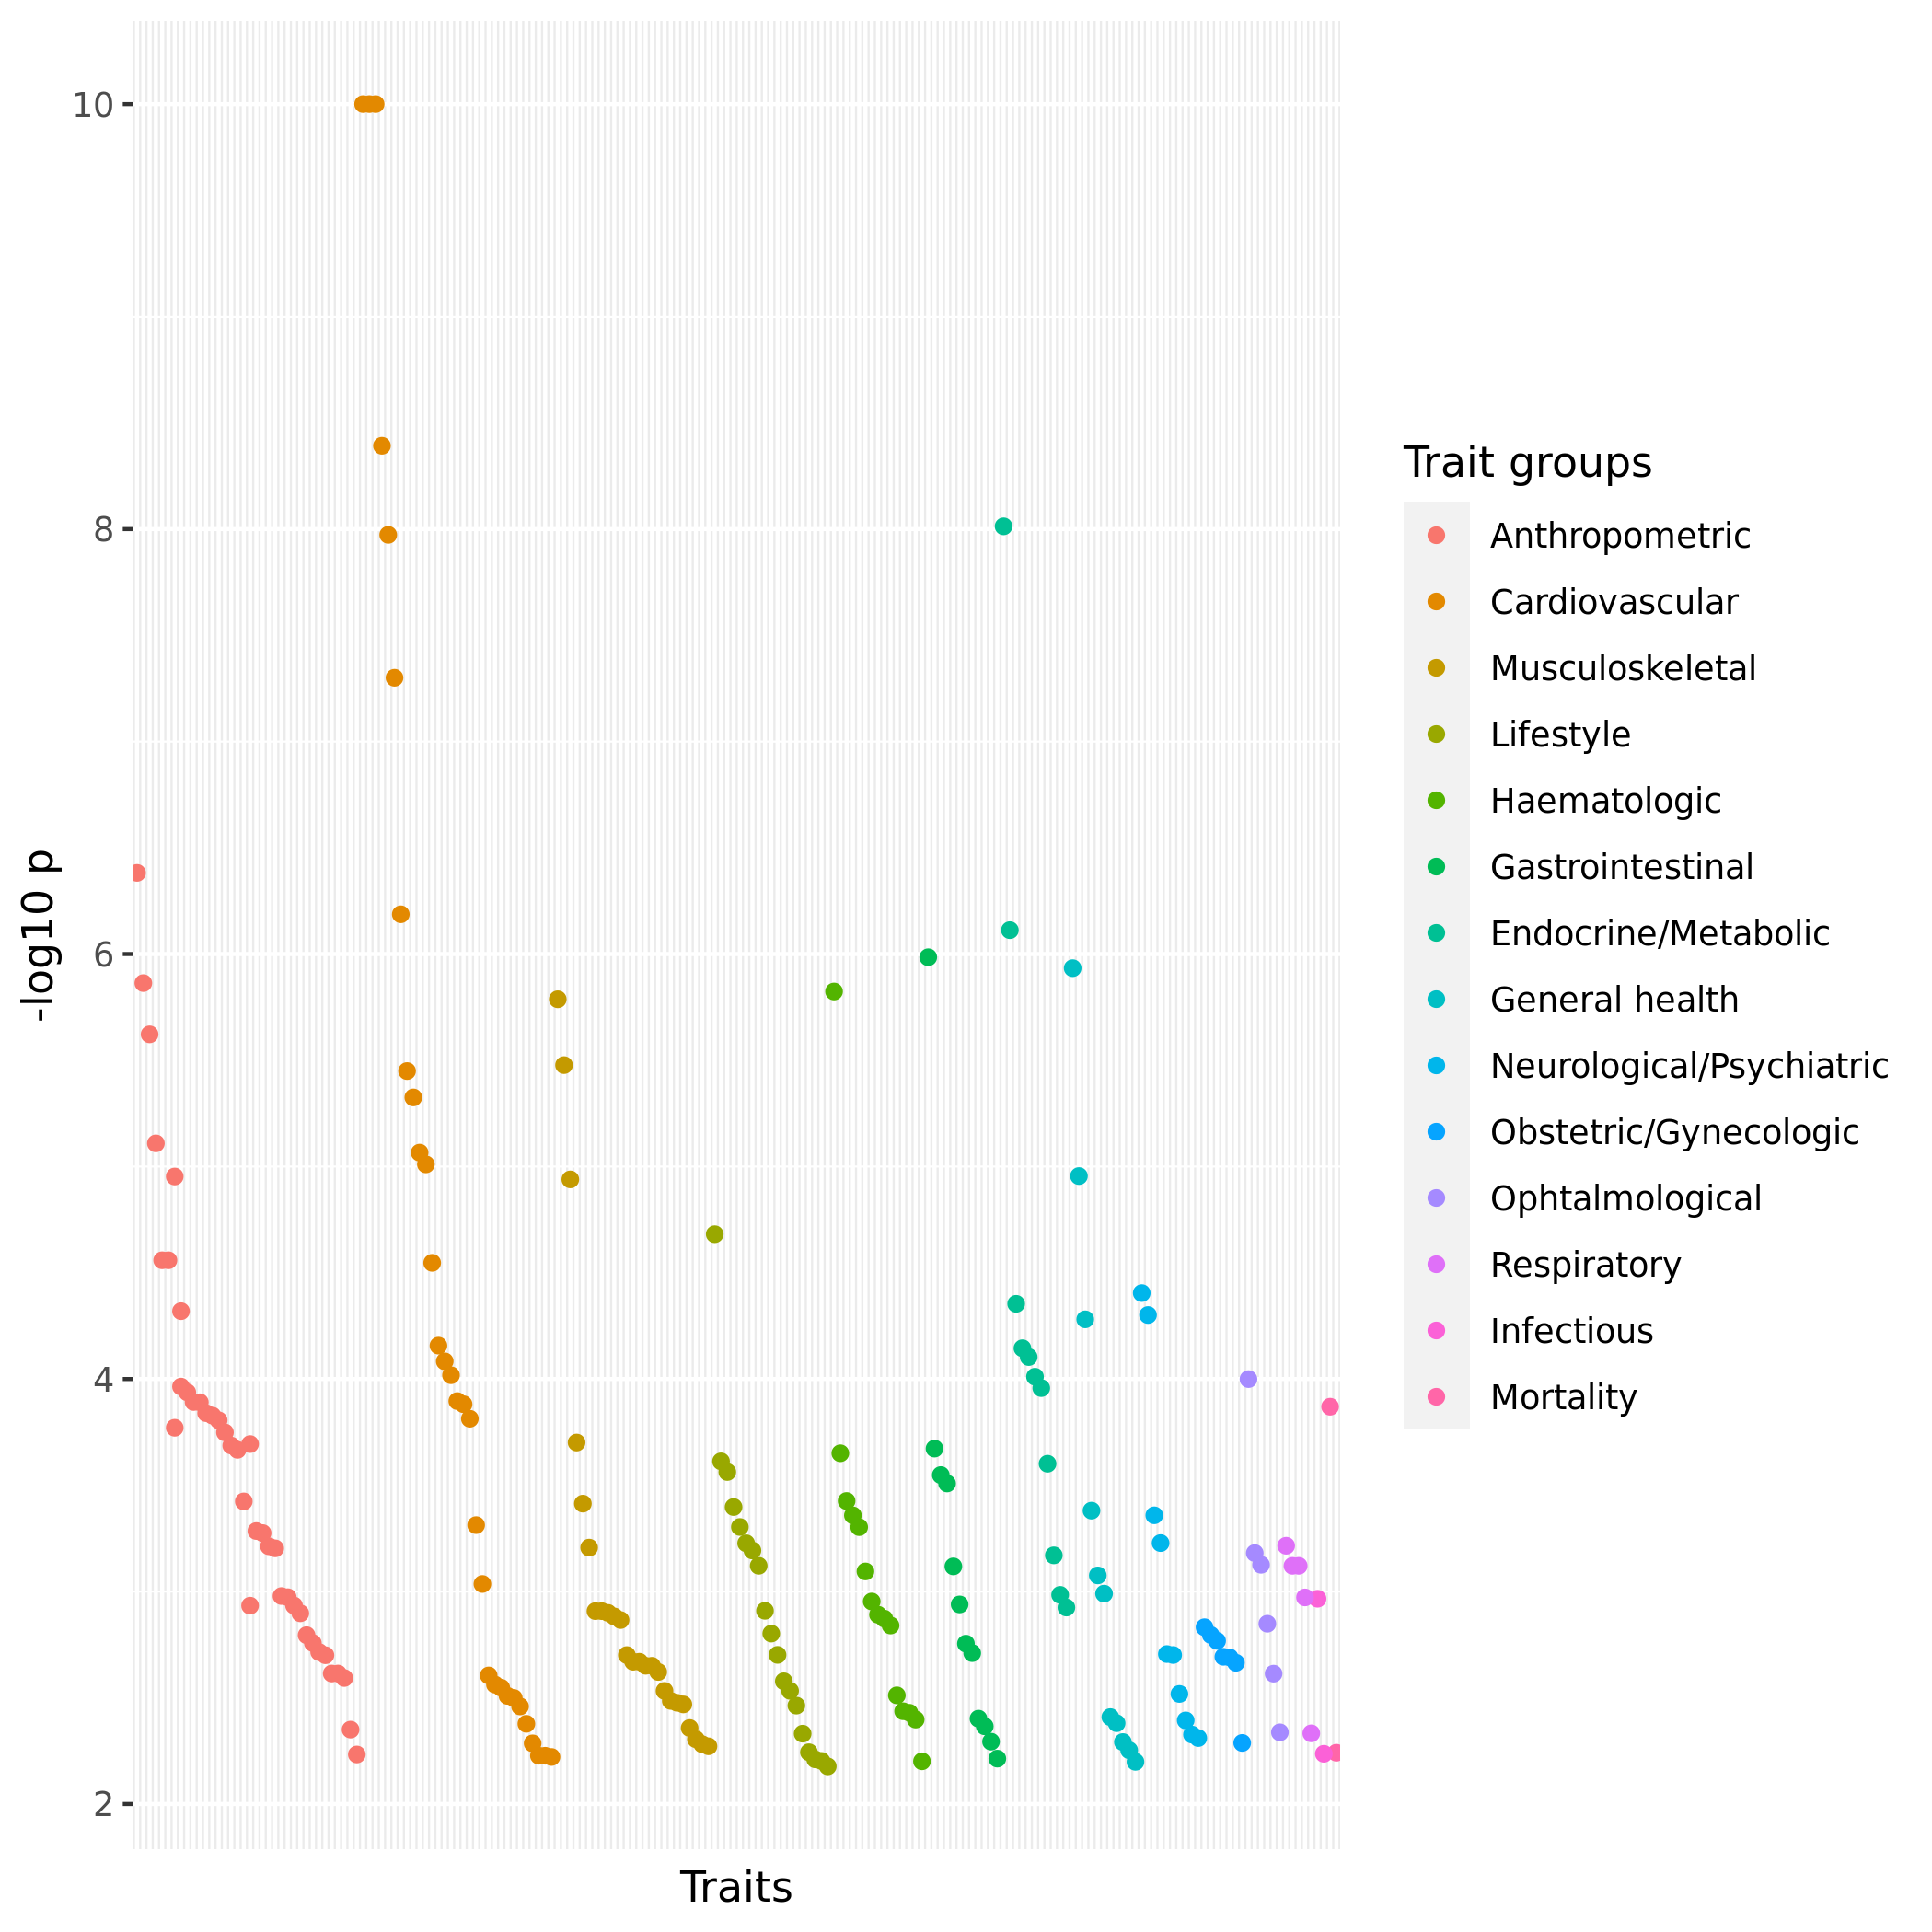
\includegraphics[width=7cm]{./plots/phewas_res.png}
\caption{Significant P values (FDR 10\%) for difference between pooled estimates (D)}
\end{figure}
\end{frame}
\begin{frame}[label={sec:orga3be5d3}]{Phenome-wide comparison - SNP-Trait matrix}
\begin{itemize}
\item For each SNP in each trait:
\end{itemize}
\begin{align*}
Z = \frac{\beta}{SE_{\beta}}
\end{align*}
\begin{itemize}
\item Produces a 67 SNP x 195 traits matrix with:
\begin{itemize}
\item High dimensionality
\item Multicolinearity
\end{itemize}
\item COVVSURF (Chavent \emph{et al.} 2019)
\begin{itemize}
\item Hierarchical agglomerative clustering - PCA
\item Random Forest
\end{itemize}
\end{itemize}
\end{frame}
\begin{frame}[label={sec:org14426a0}]{PCA}
\begin{itemize}
\item PCs are linear combinations of original variables
\begin{itemize}
\item Redundant variables can be summarized
\item The contribution of a variable in a PC = Squared loading (Pearson's \emph{r\textsuperscript{2}})
\end{itemize}
\item Maximum possible information (variance) is summarized in PC1
\end{itemize}
\end{frame}
\begin{frame}[label={sec:org71db267}]{Random Forest (RF)}
\begin{itemize}
\item Multiple decision trees - Classification or regression
\begin{itemize}
\item Grown using a random subset of columns and rows of the original data (in-bag)
\begin{itemize}
\item Replacement
\end{itemize}
\item Tested using out-of-bag (OOB) data
\begin{itemize}
\item Estimation of error rate / accuracy
\end{itemize}
\end{itemize}
\item The output includes:
\begin{itemize}
\item Probability (\emph{votes})/value assigned by trees
\item Importance score
\begin{itemize}
\item Error rate increase if variable is absent
\end{itemize}
\item Proximity matrix
\begin{itemize}
\item N times two observations occupy the same terminal node
\item From Breiman and Cutler:
\end{itemize}
\end{itemize}
\end{itemize}
\begin{center}
\emph{\(1 - prox(n_i,n_j)\) are squared distances in a Euclidean space}
\end{center}
\end{frame}
\begin{frame}[label={sec:org35ecae5}]{Clustering of traits using RF}
\begin{itemize}
\item Dimensionality reduction into clusters of traits
\item Relevant for distinguishing between the two sets of SNPs
\item Non-parametric, data-driven
\item Process:
\begin{enumerate}
\item Agglomerative clustering using PCA results in:
\begin{itemize}
\item Clustering tree with \emph{k} = 1,2,3\ldots{}/p/ possible partitions
\item At every \emph{k}: the 1PCs summarize each cluster
\end{itemize}
\item Among every \emph{k}: 1PC as predictors for RF
\item Model with minimum OOB error rate determines the optimal \emph{k}.
\item Nested RF models
\begin{itemize}
\item Starting with model with only the most important cluster
\item Ending with model including all clusters selected in \alert{3}
\item Final model - minimum OOB error rate
\end{itemize}
\end{enumerate}
\end{itemize}
\end{frame}
\begin{frame}[label={sec:orgd4c7cd4}]{RF models}
\begin{figure}[htbp]
\centering
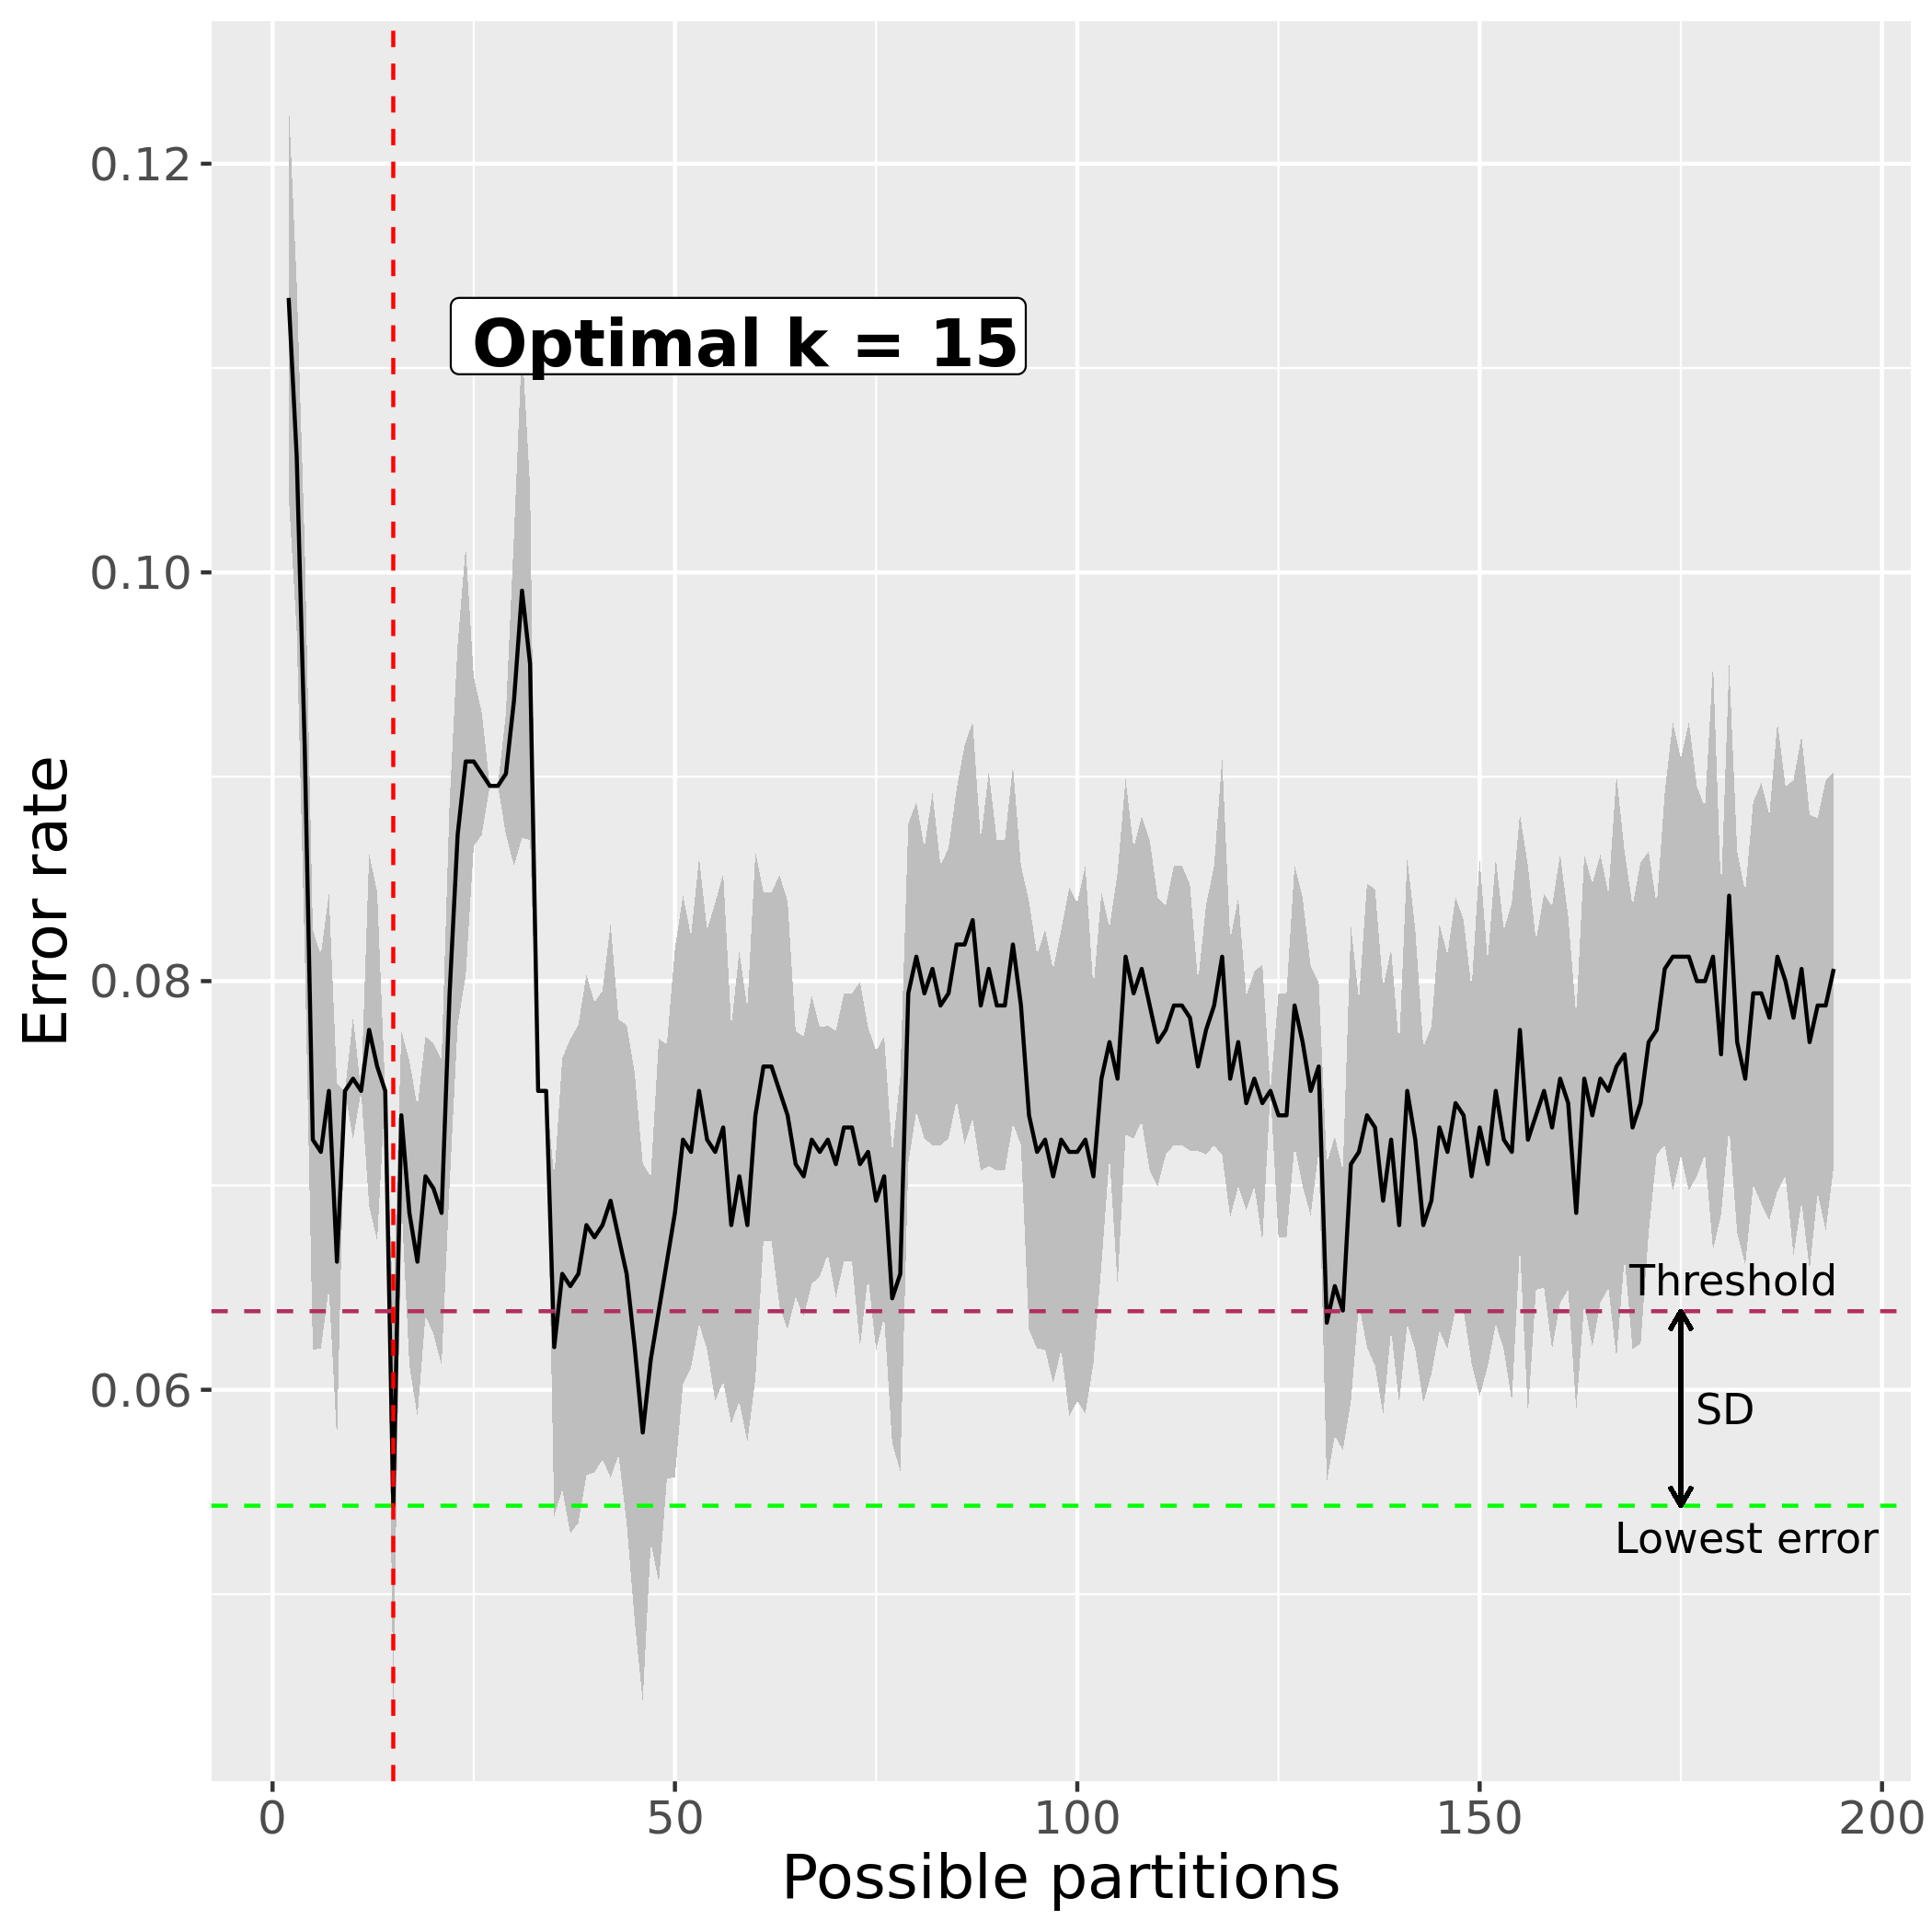
\includegraphics[width=7cm]{./plots/kopt_phen.png}
\caption[\emph{k}]{Error rate of RF models across every \emph{k}}
\end{figure}
\end{frame}
\begin{frame}[label={sec:org09586ba}]{Clusters}
\begin{figure}[htbp]
\centering
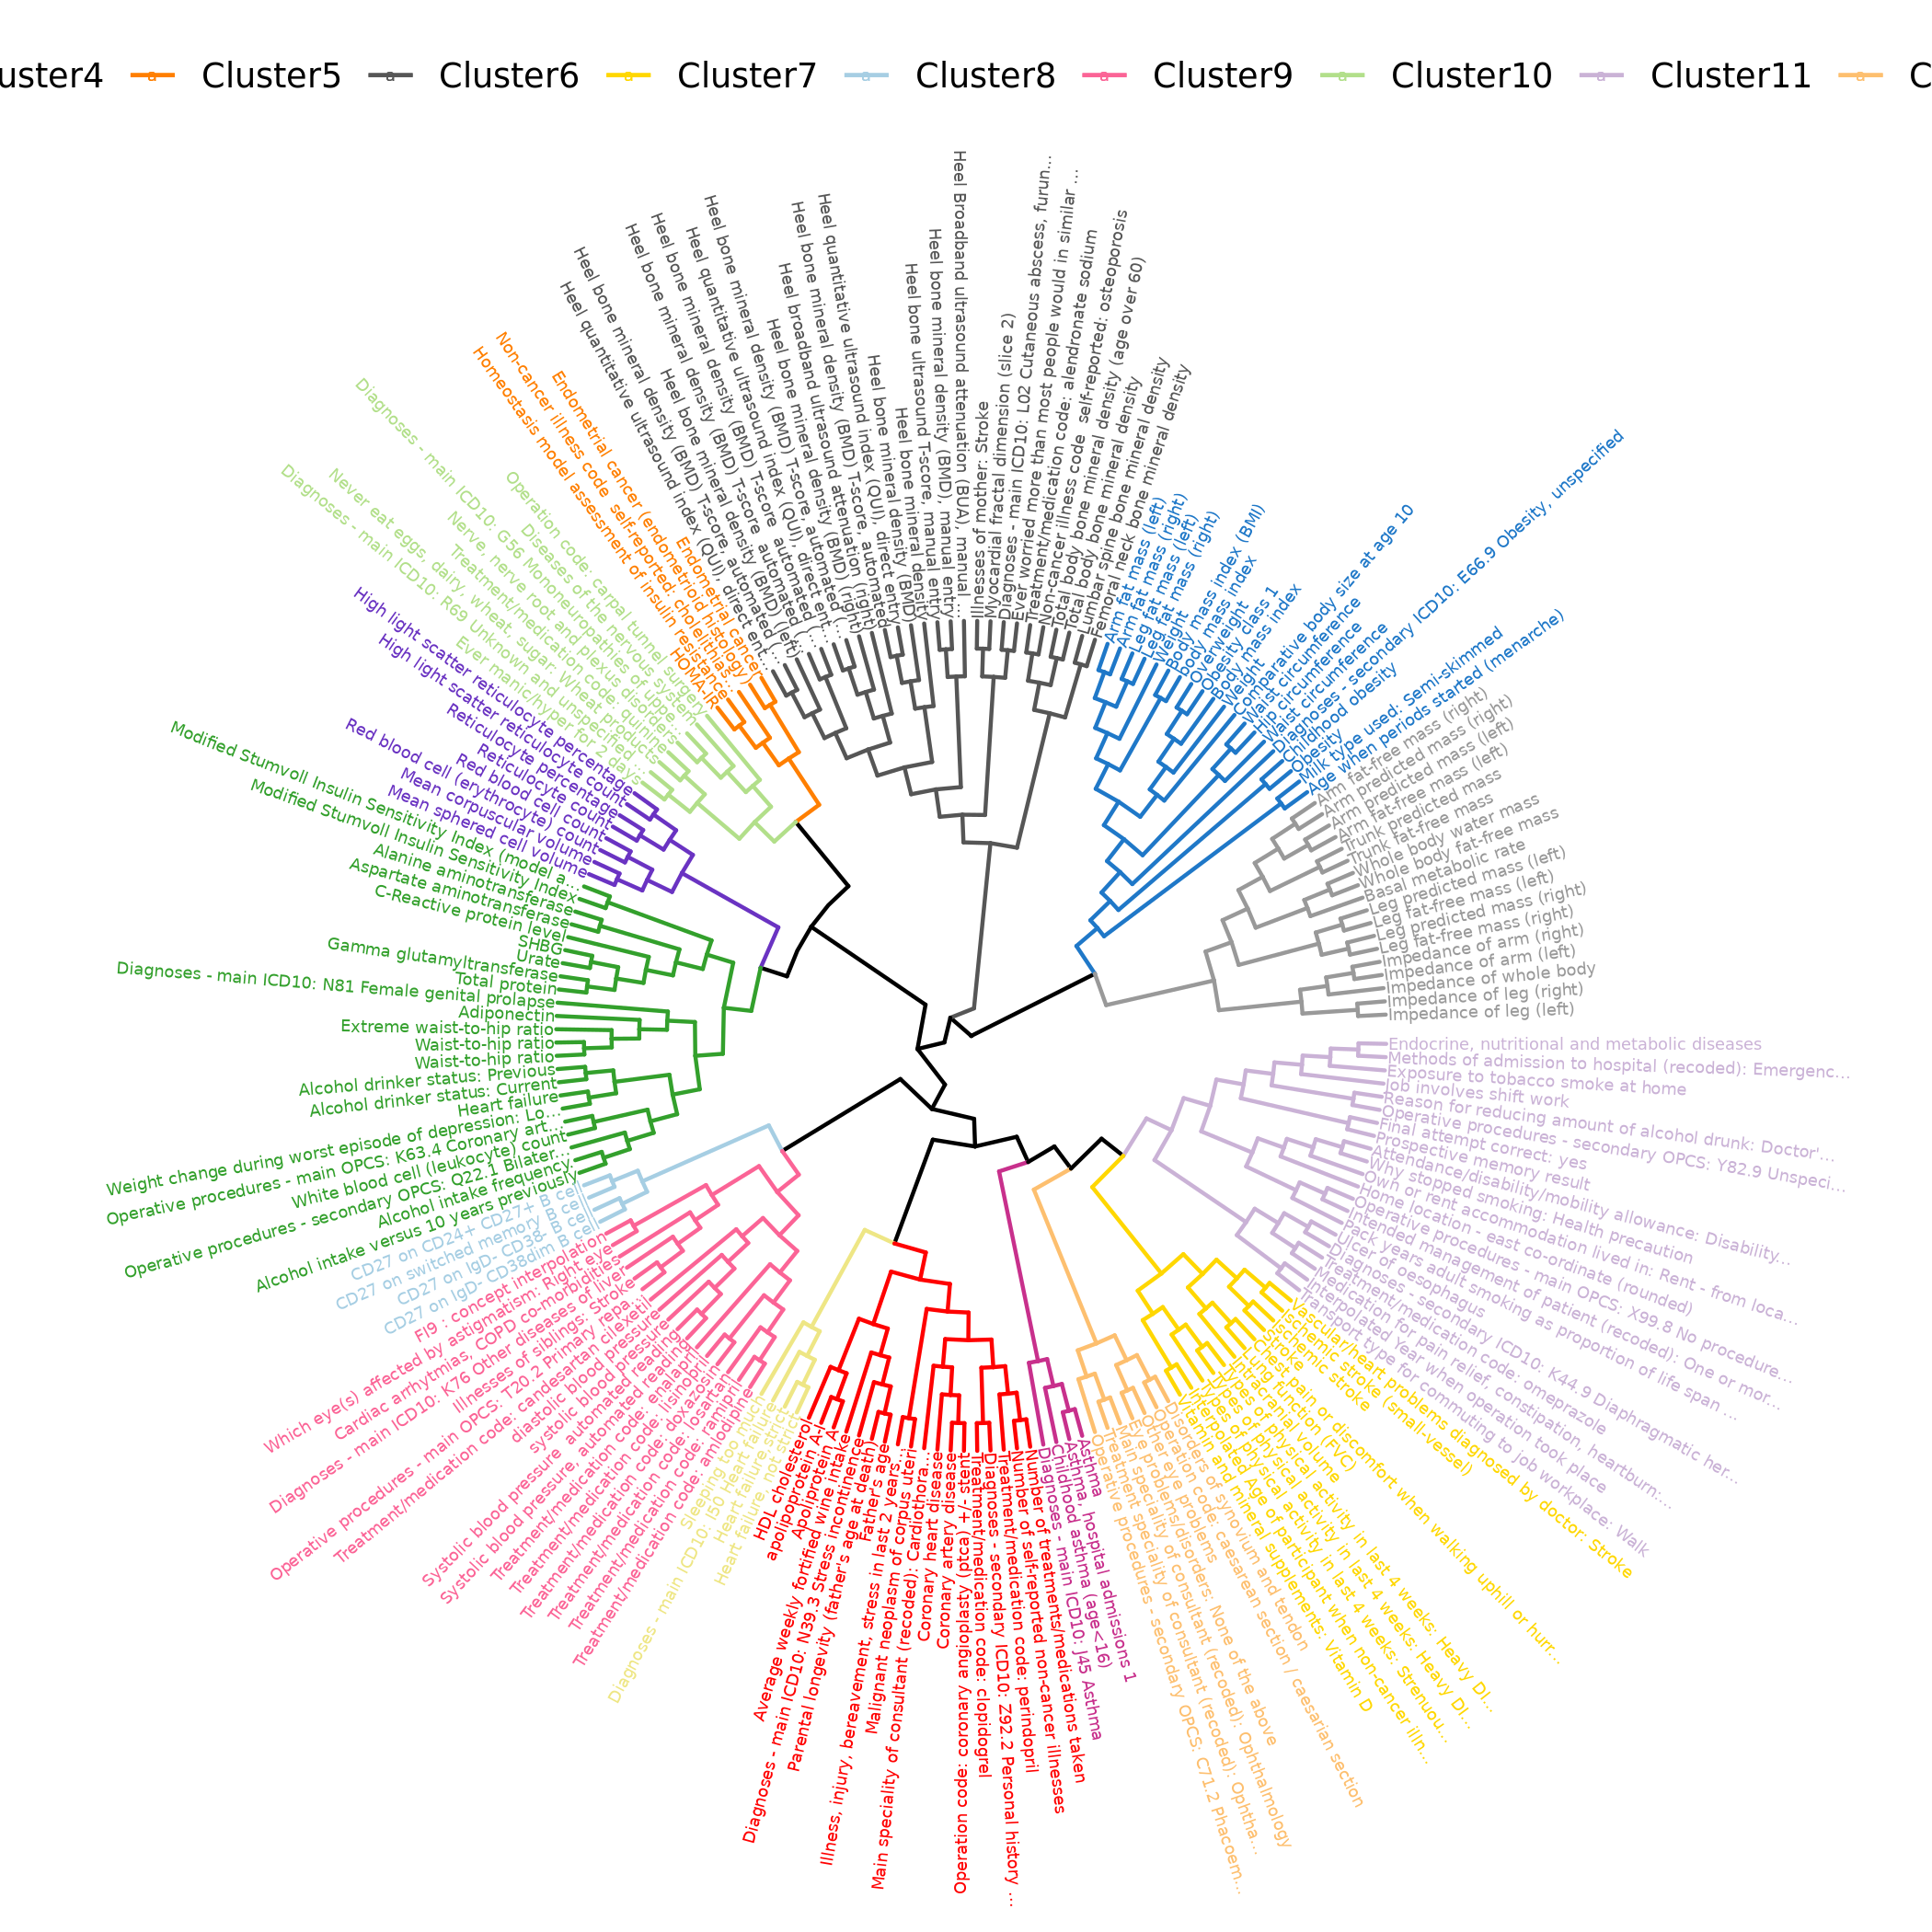
\includegraphics[width=7cm]{./plots/dend_phen.png}
\caption{Clustering tree with optimal partition}
\end{figure}
\end{frame}
\begin{frame}[label={sec:org141a6cb}]{Trait selection - First stage}
\begin{figure}[htbp]
\centering
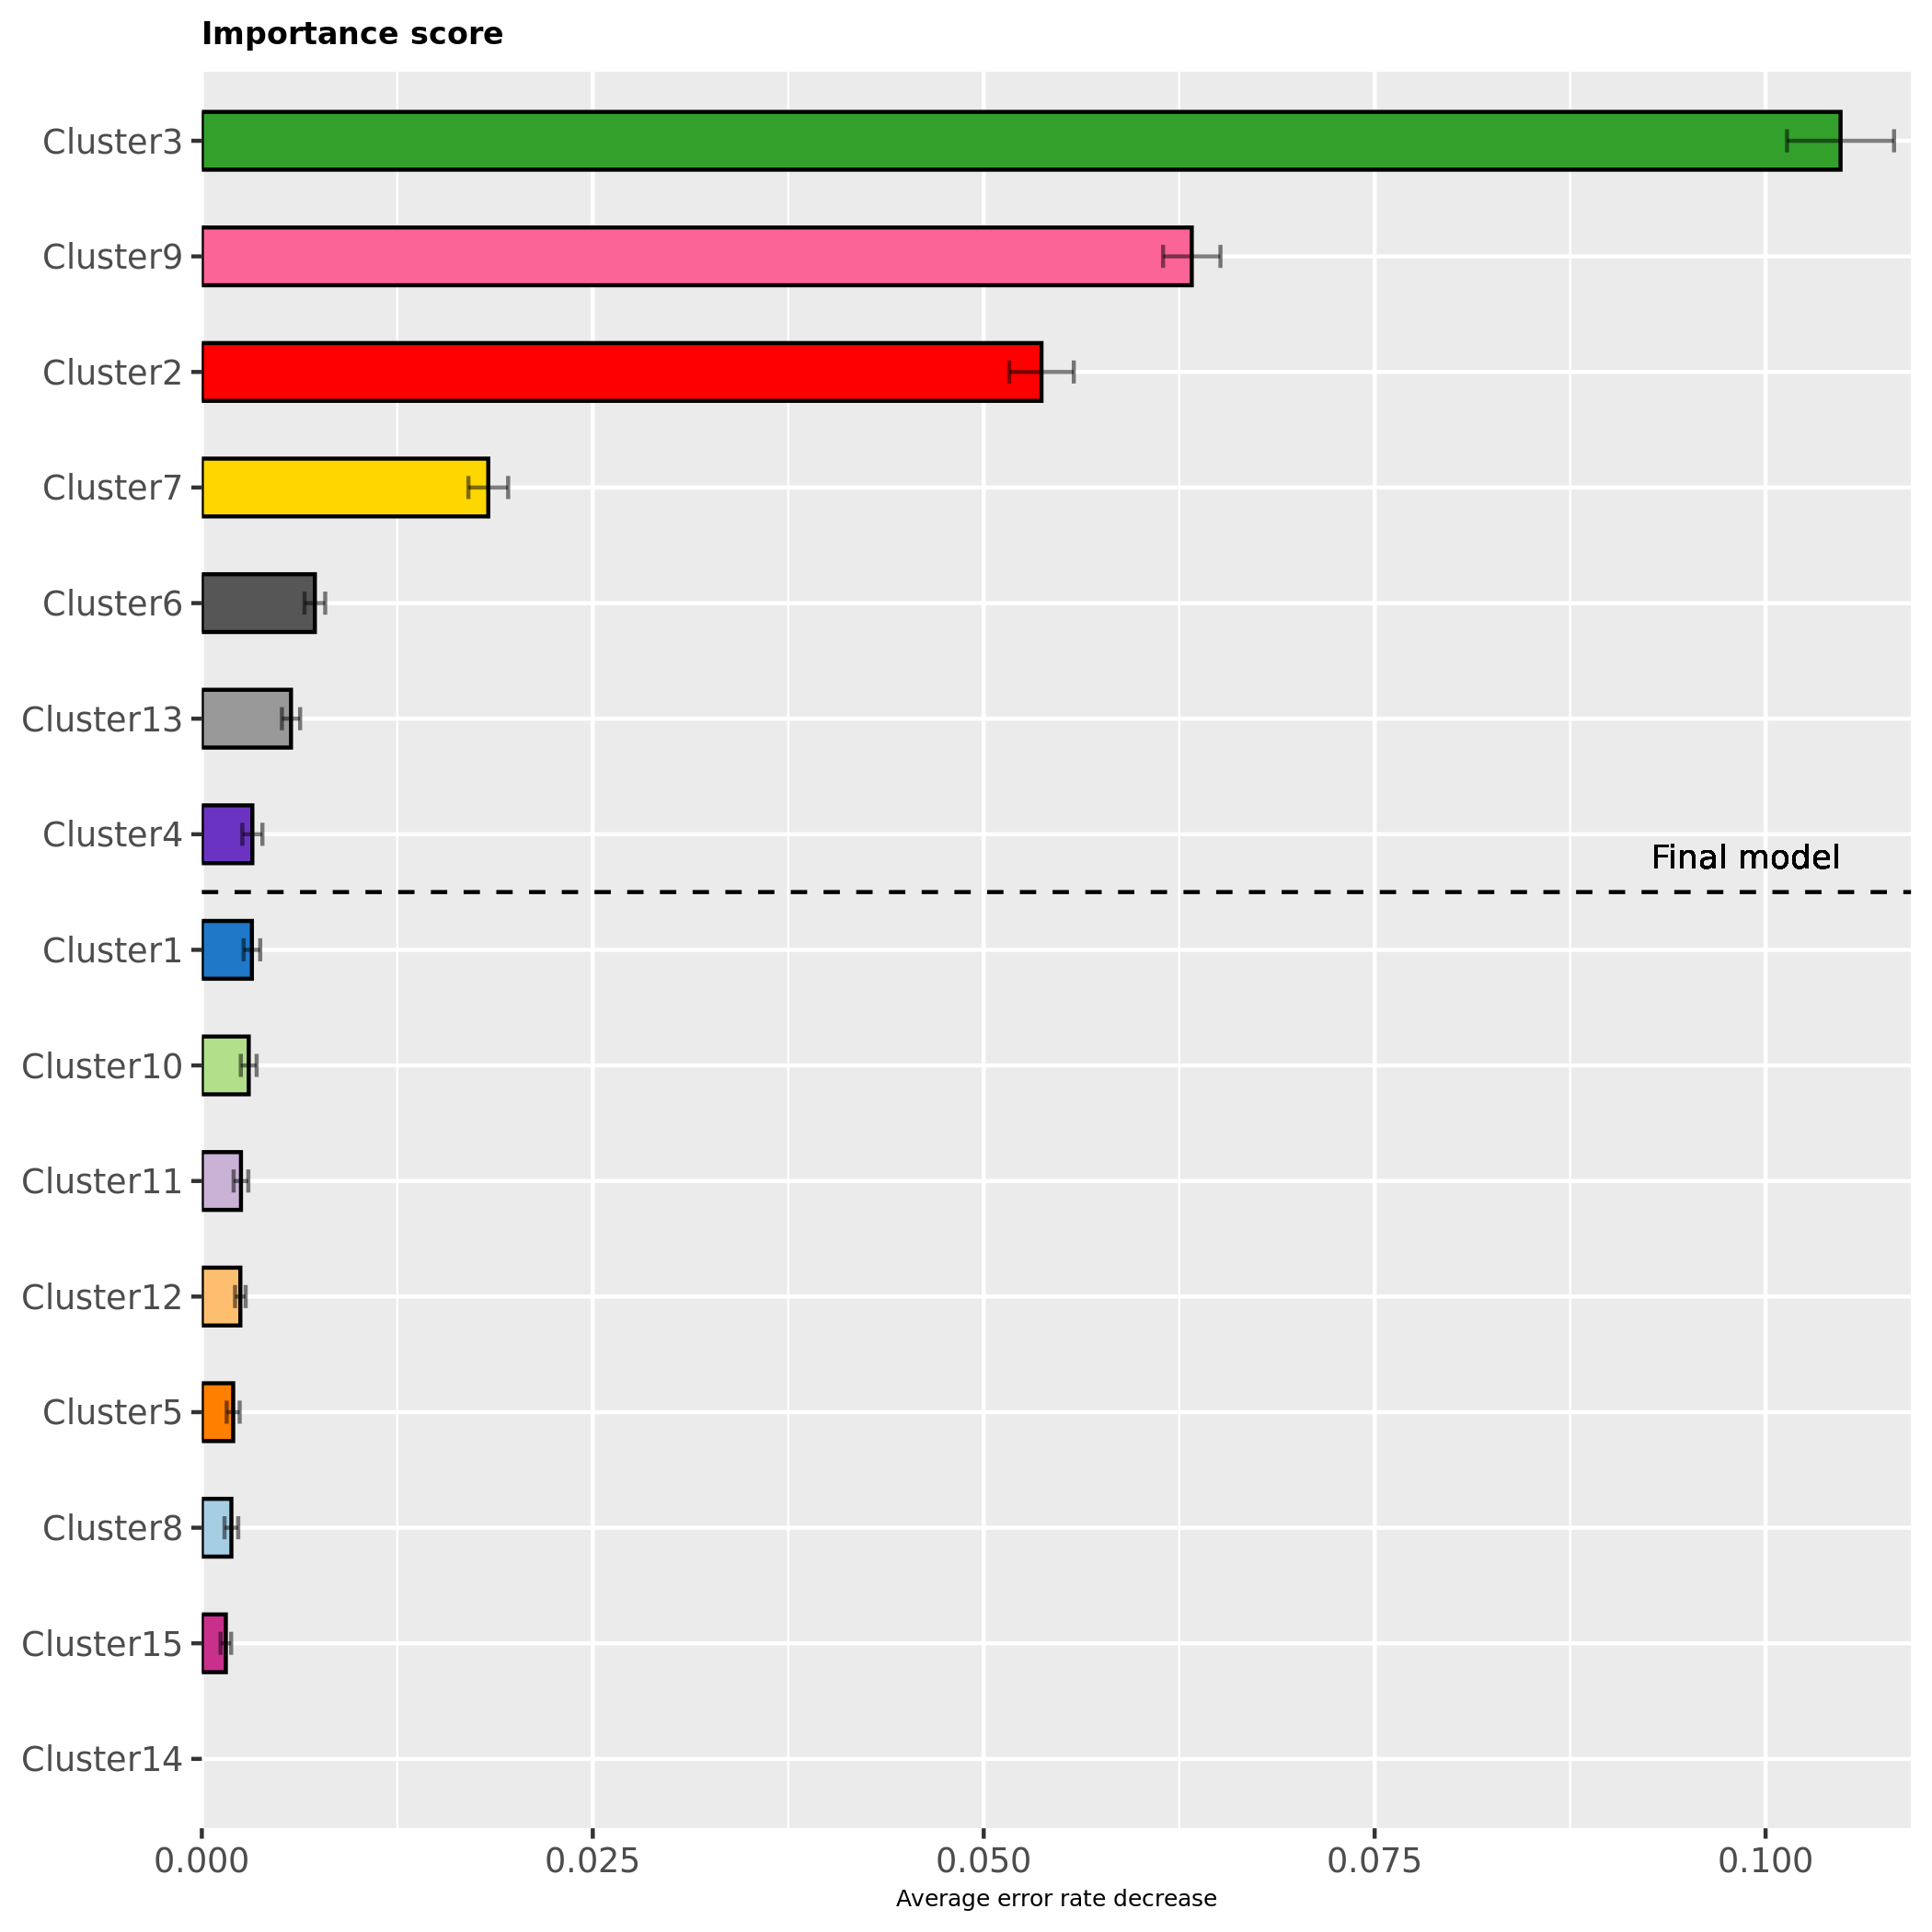
\includegraphics[width=7cm]{./plots/clusimp_phen.png}
\caption{Importance score of clusters}
\end{figure}
\end{frame}
\begin{frame}[label={sec:org7281a03}]{Trait selection - Final model}
\begin{figure}[htbp]
\centering
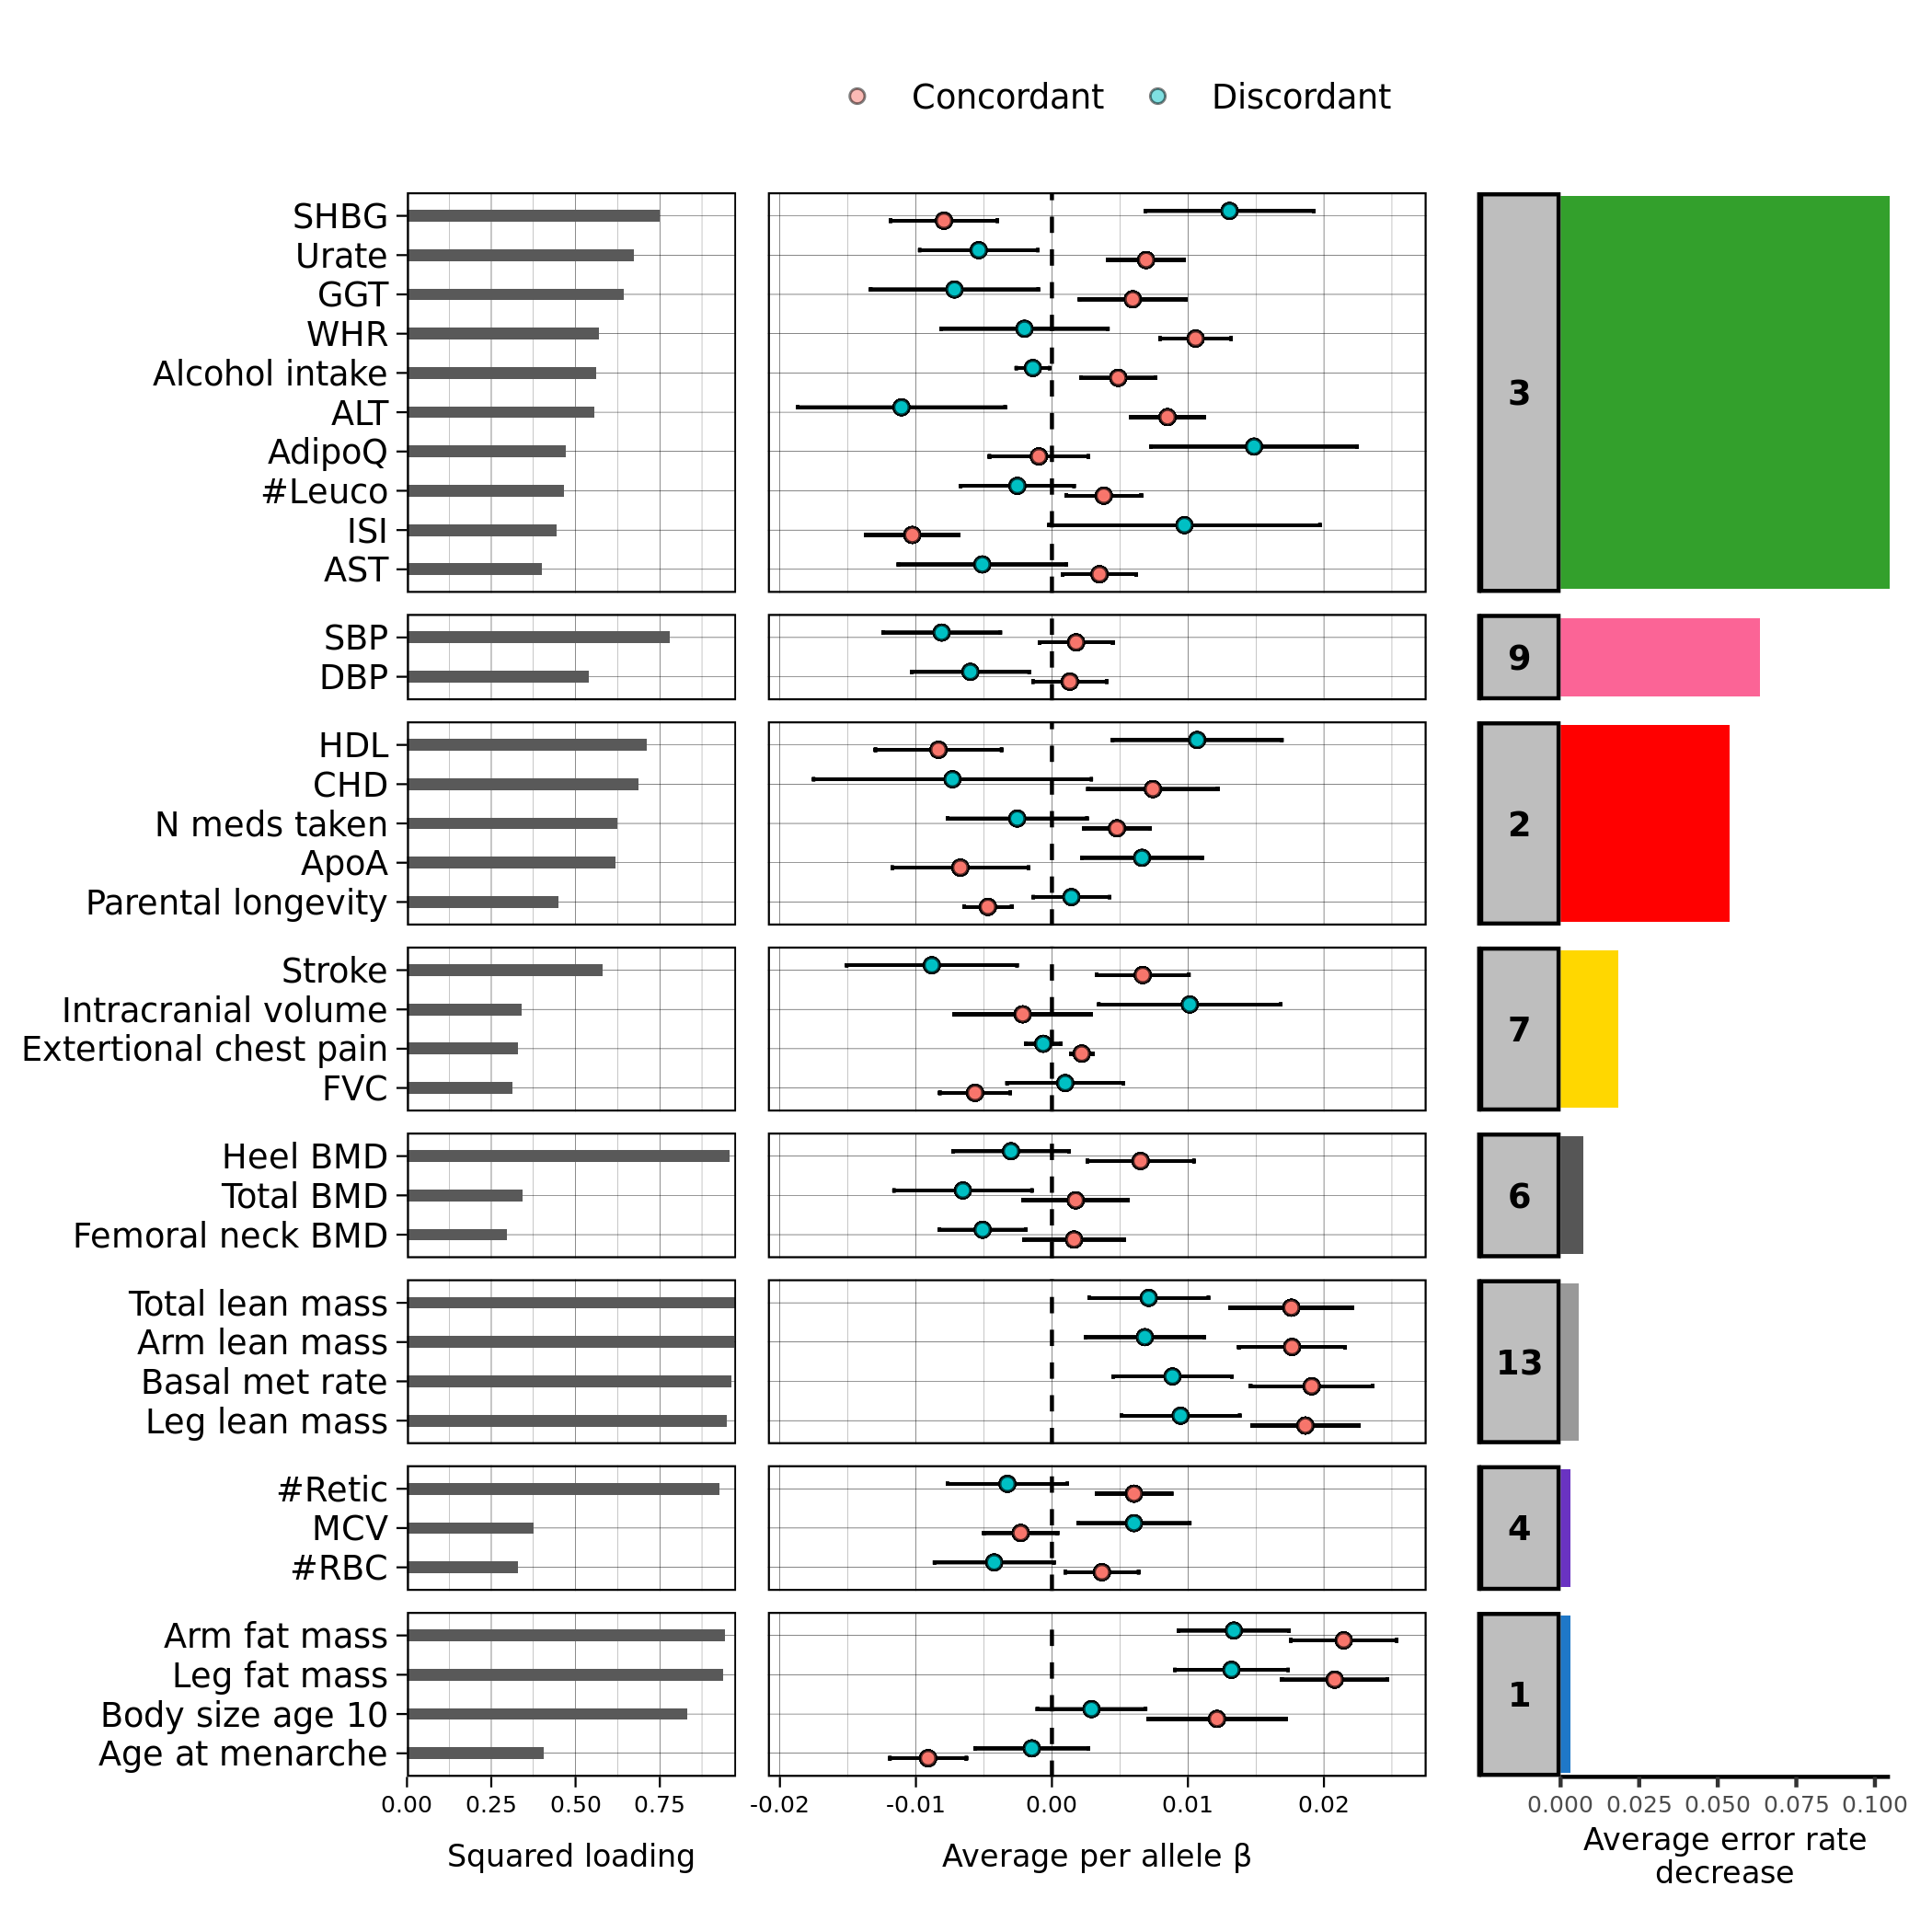
\includegraphics[width=7cm]{./plots/clus_str_phen.png}
\caption{Importance score, squared loading and pooled estimates of each subtype}
\end{figure}
\end{frame}
\begin{frame}[label={sec:org7ccbeec}]{Main variables}
\begin{figure}[htbp]
\centering
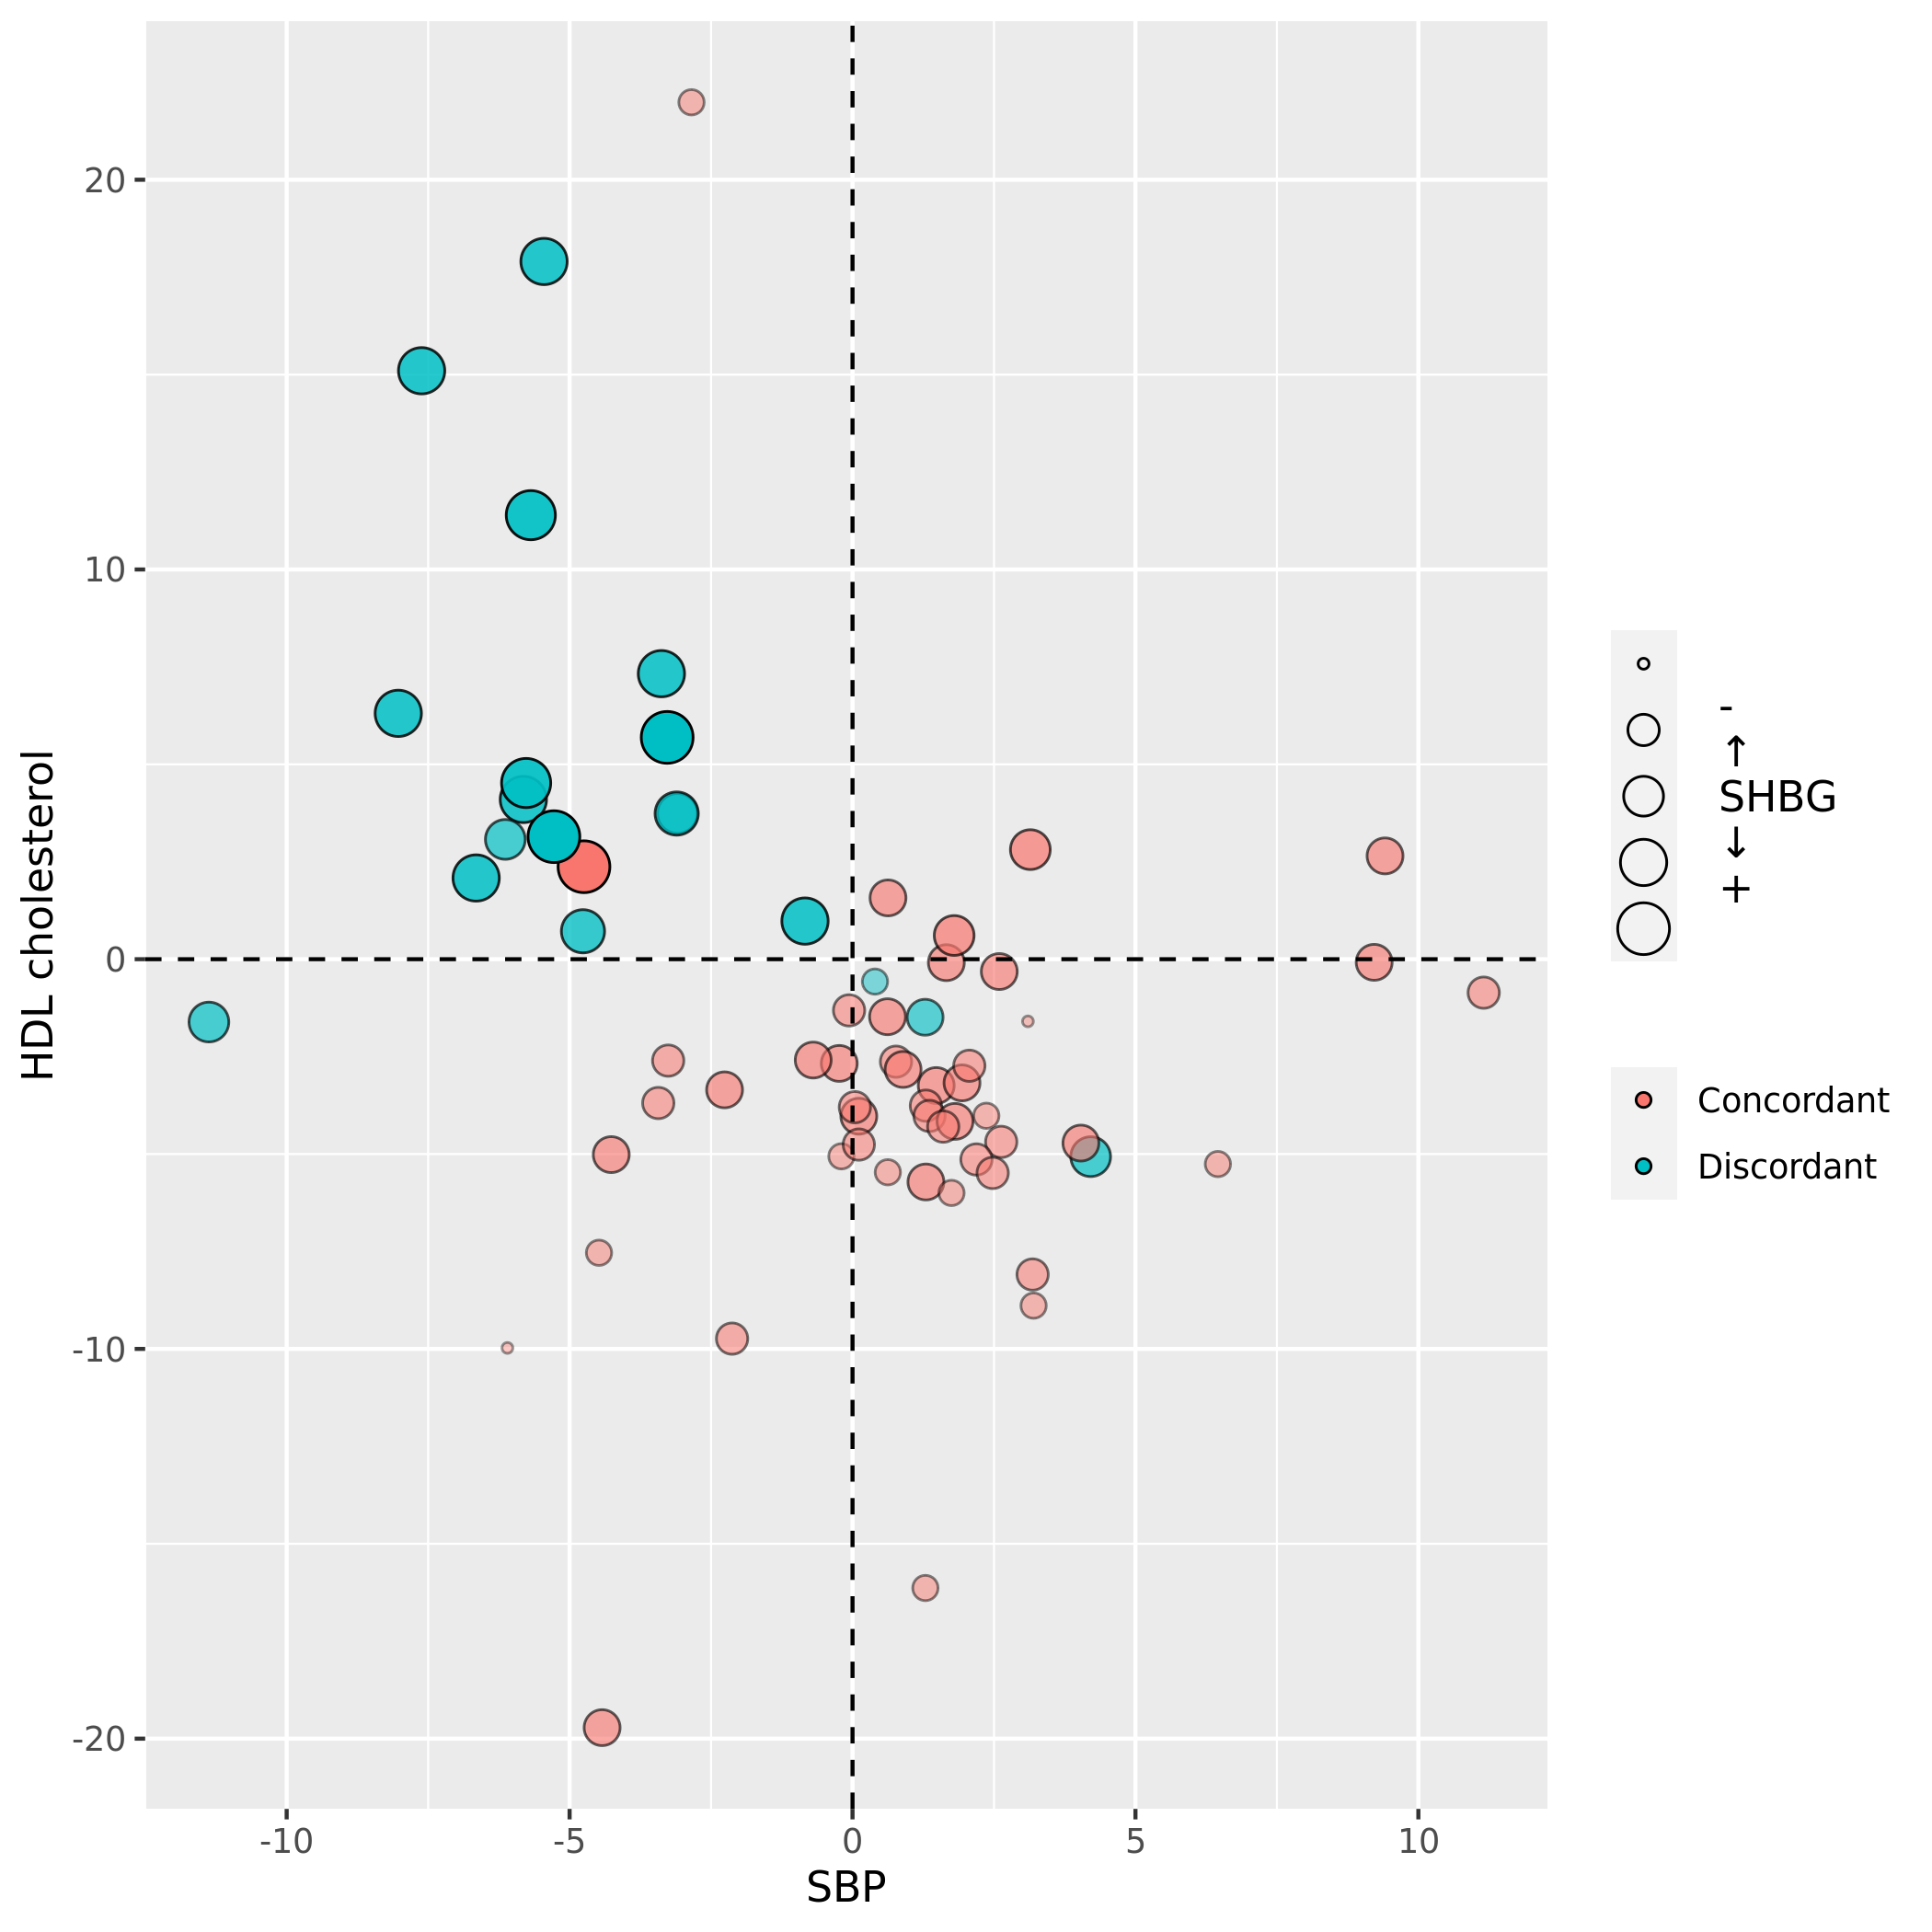
\includegraphics[width=7cm]{./plots/mainvars_phen.png}
\caption{SNP effects for the main three variables}
\end{figure}
\end{frame}
\begin{frame}[label={sec:orga95c470}]{Proximity matrix}
\begin{figure}[htbp]
\centering
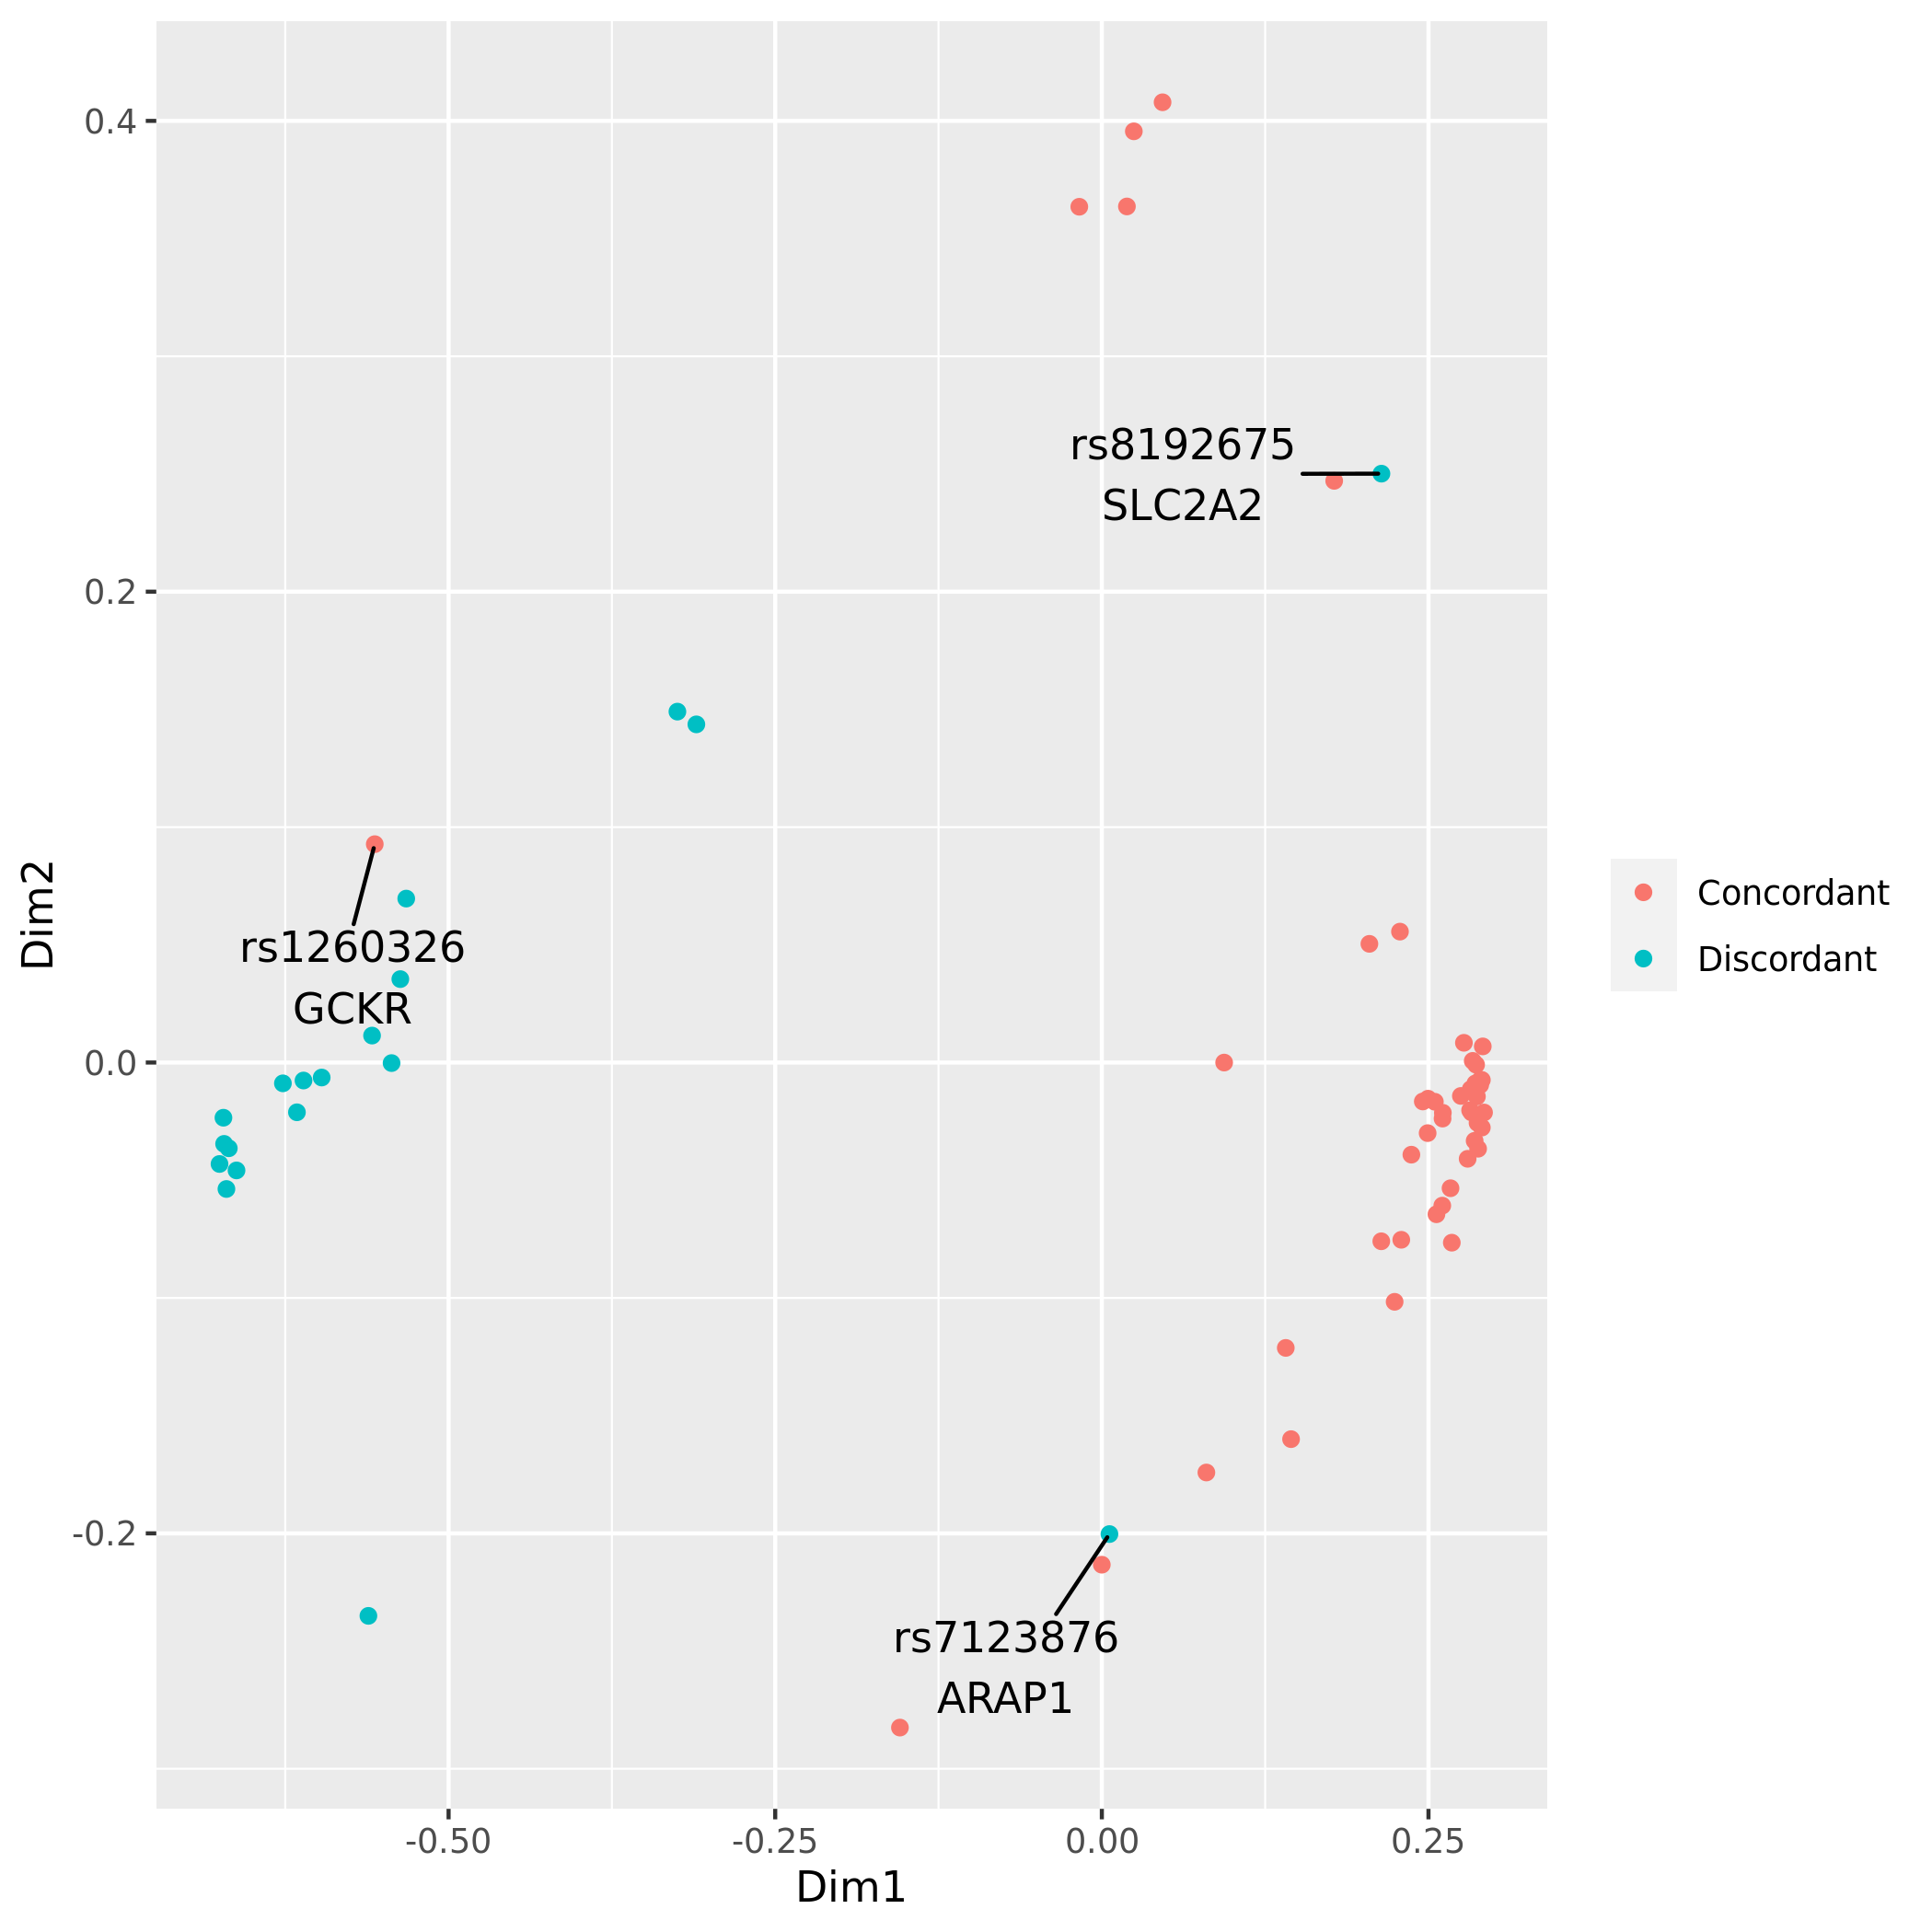
\includegraphics[width=7cm]{./plots/mds_phen.png}
\caption{Multi-dimensional scaling of RF proximity matrix}
\end{figure}
\end{frame}
\begin{frame}[label={sec:org55828af}]{Individual SNP effects on traits selected}
\begin{figure}[htbp]
\centering
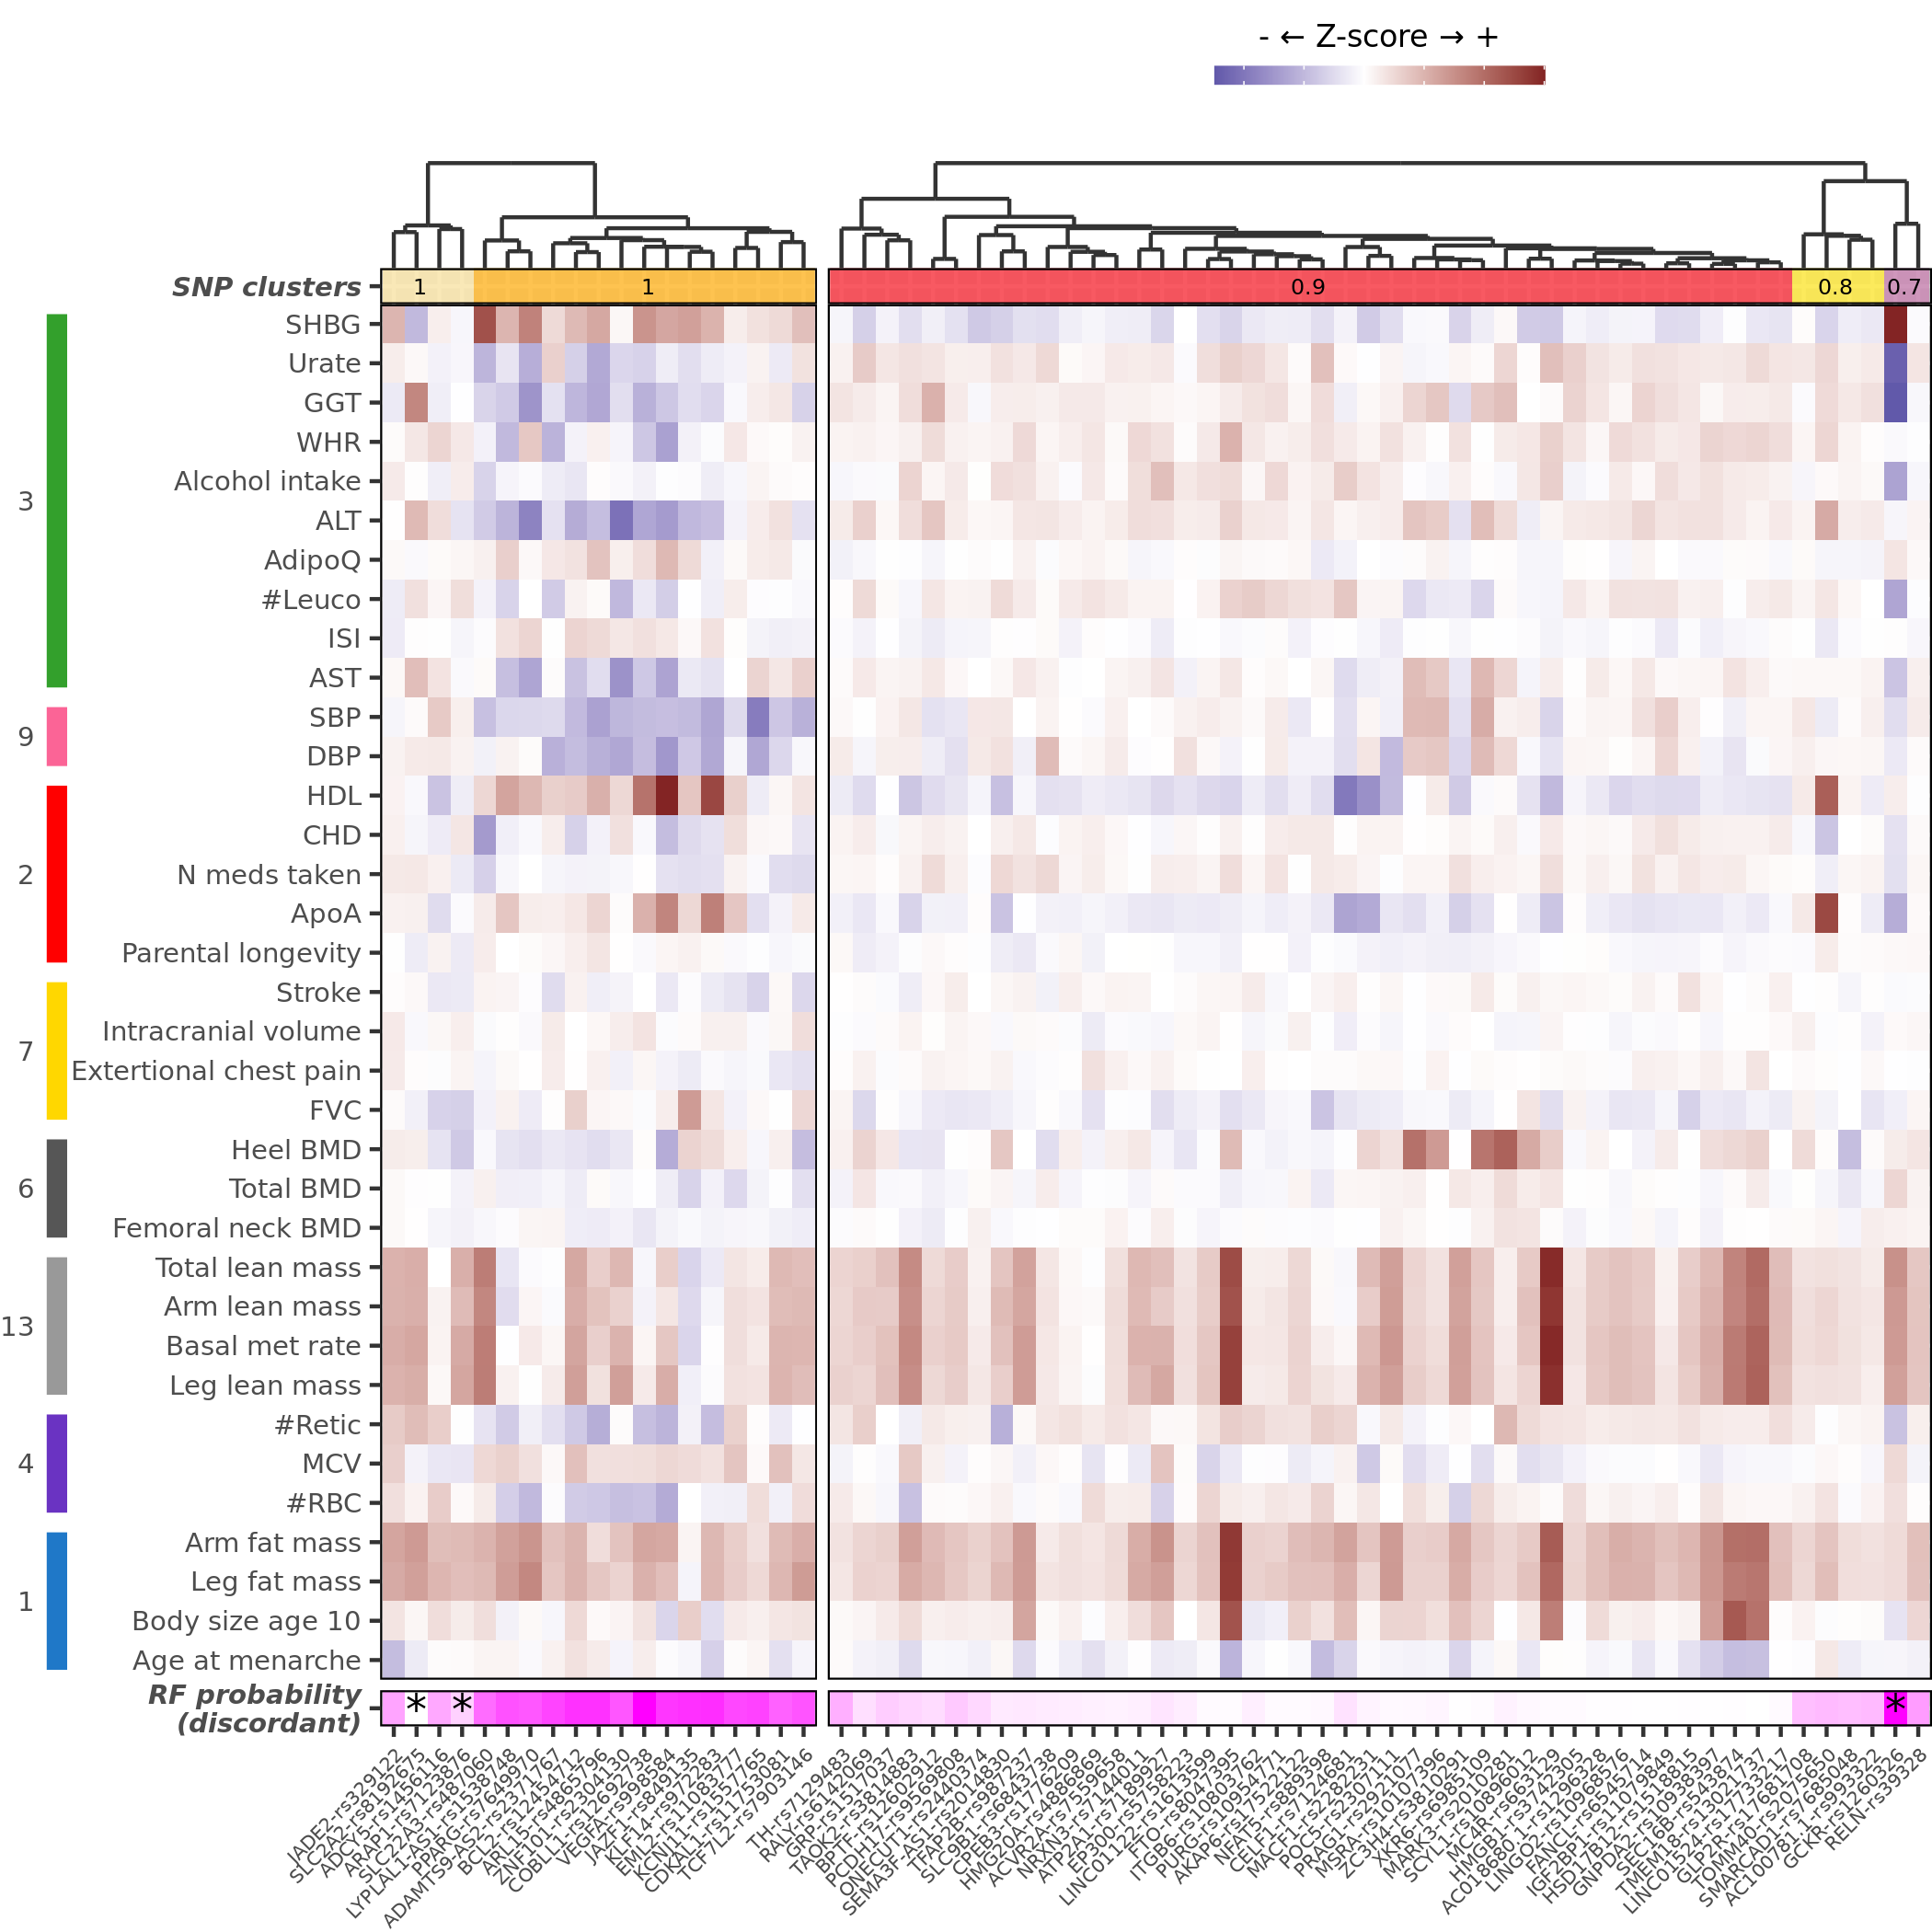
\includegraphics[width=7cm]{./plots/phen_hm.png}
\caption{Heatmap of main variables and RF assignment}
\end{figure}
\end{frame}
\begin{frame}[label={sec:org3c67eb1}]{External validation - BioVU PheWAS}
\begin{figure}[htbp]
\centering
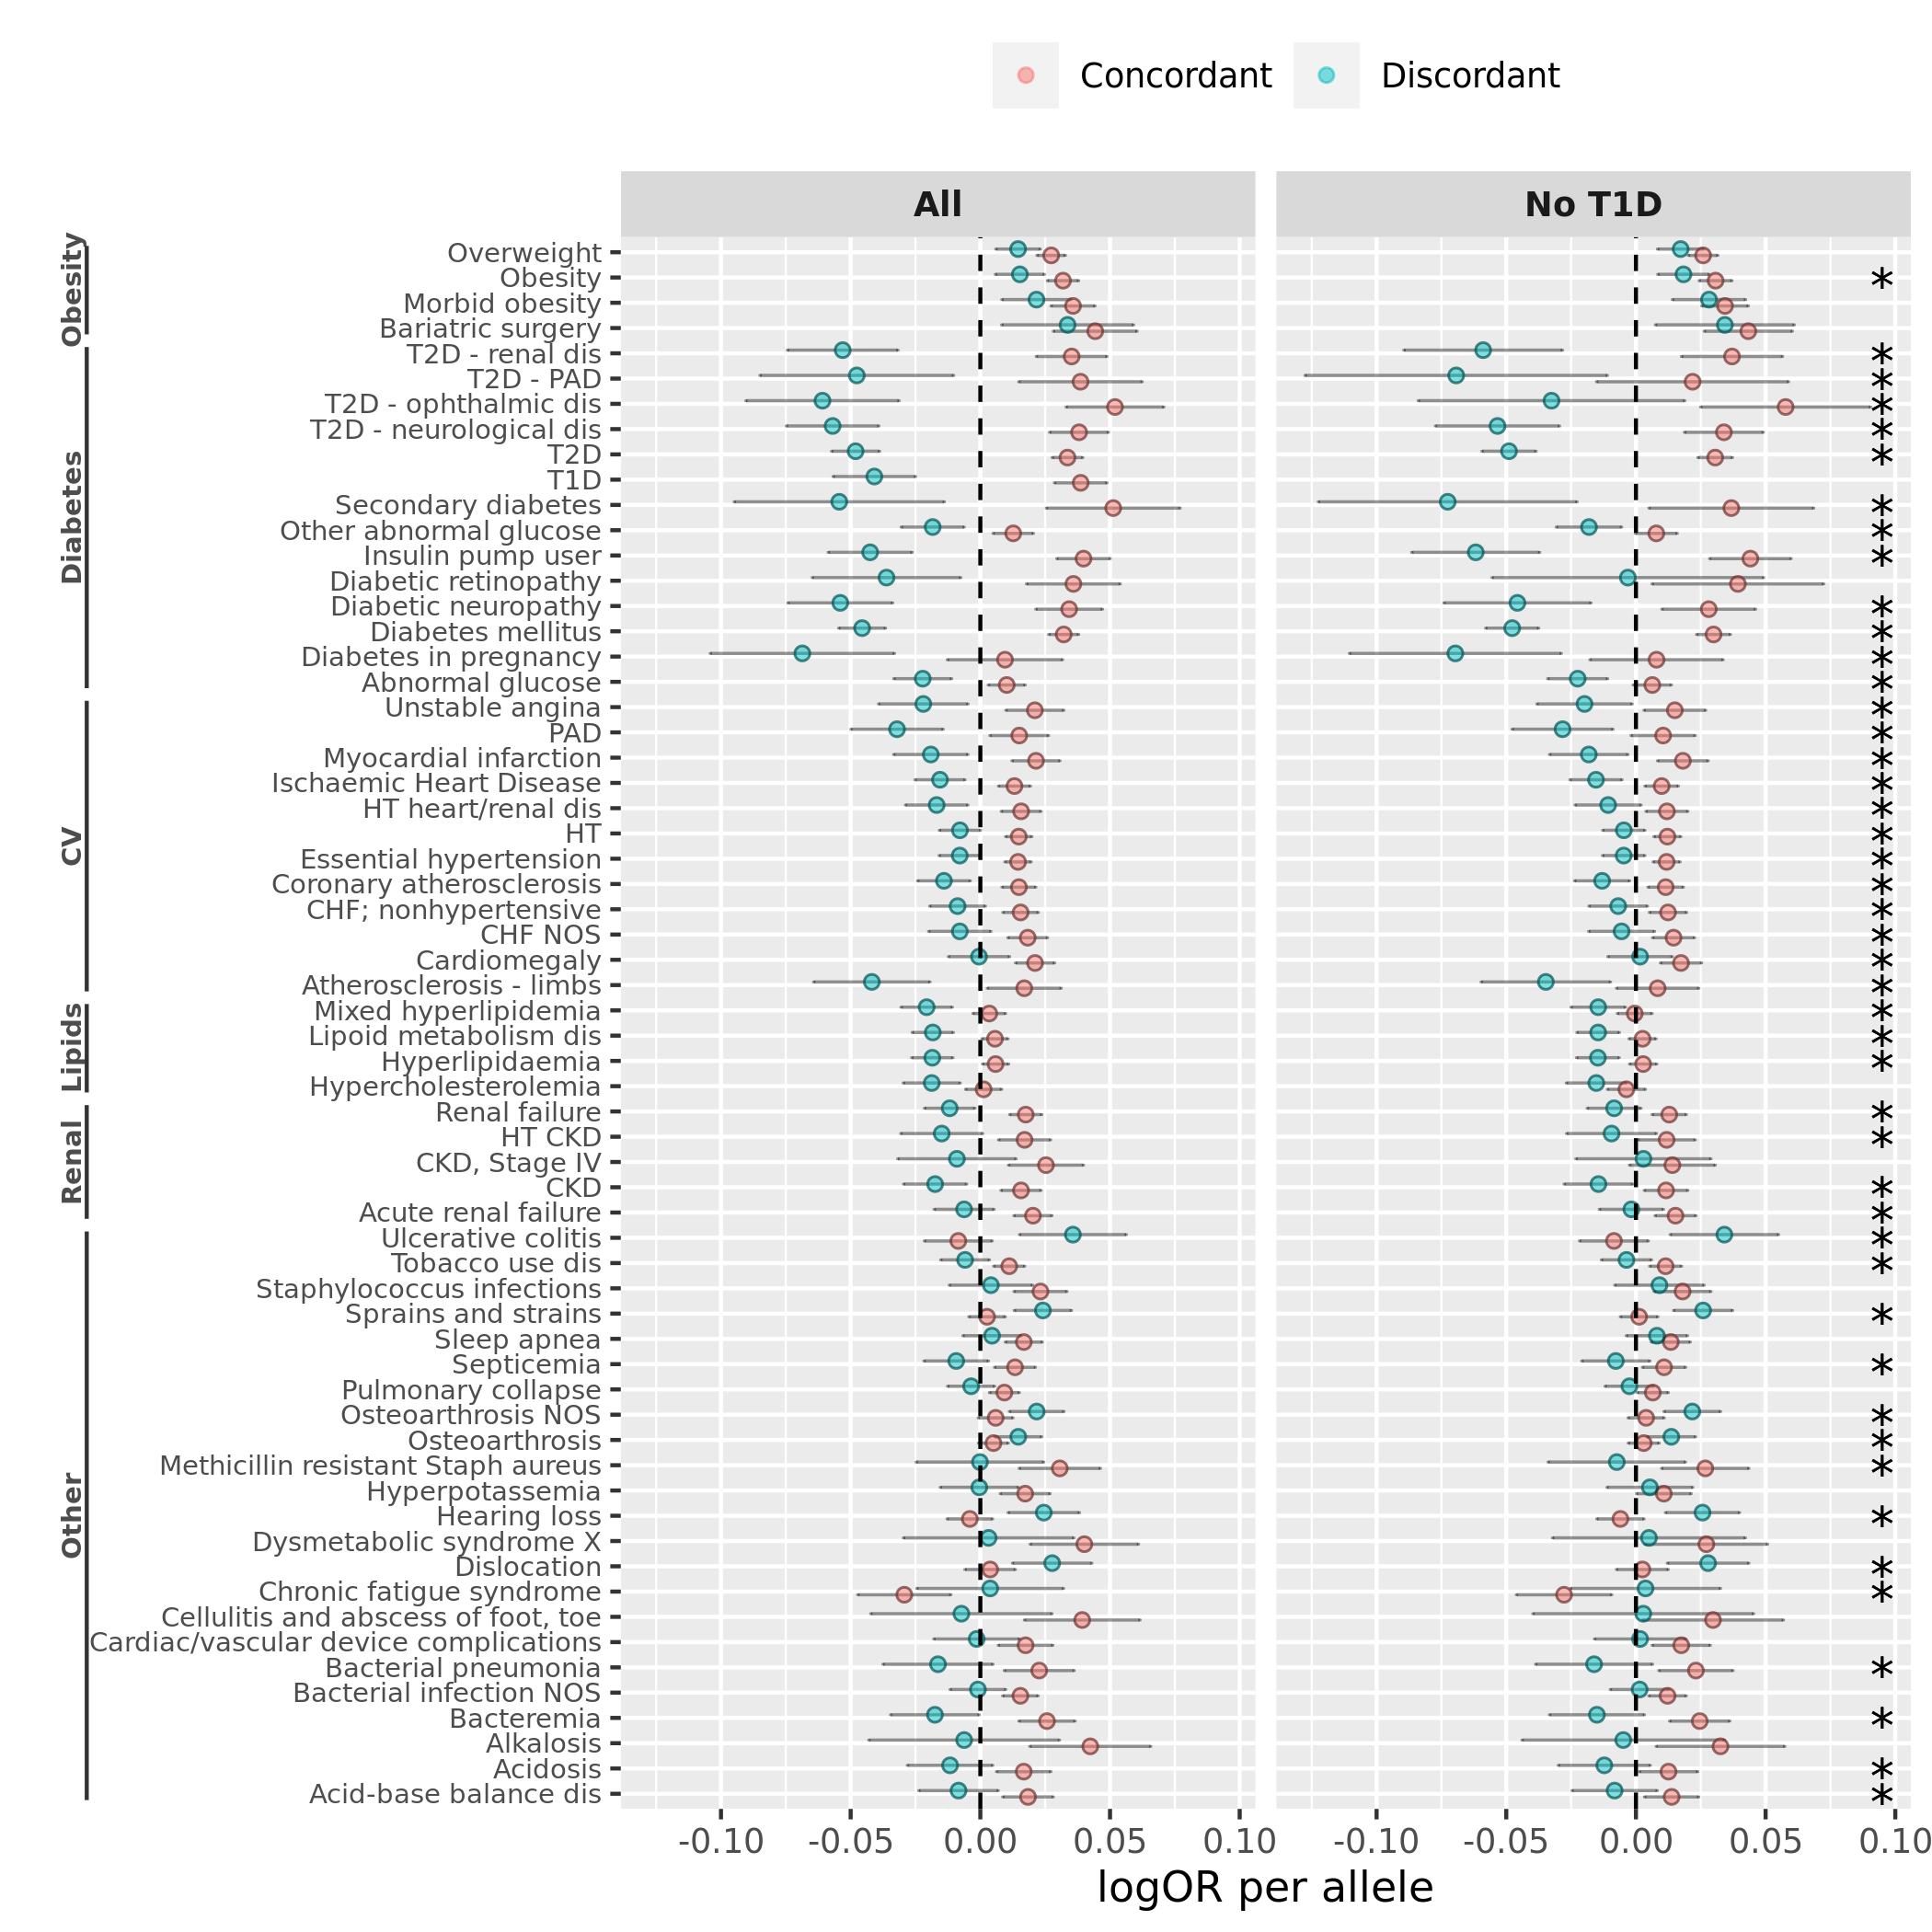
\includegraphics[width=7cm]{./plots/biovu_pw.png}
\caption{Concordant and discordant effects in BioVU. Stars represent 5\% FDR significance after exclusion of individuals with T1D}
\end{figure}
\end{frame}
\begin{frame}[label={sec:orgf9915d8}]{External validation - BioVU LabWAS}
\begin{figure}[htbp]
\centering
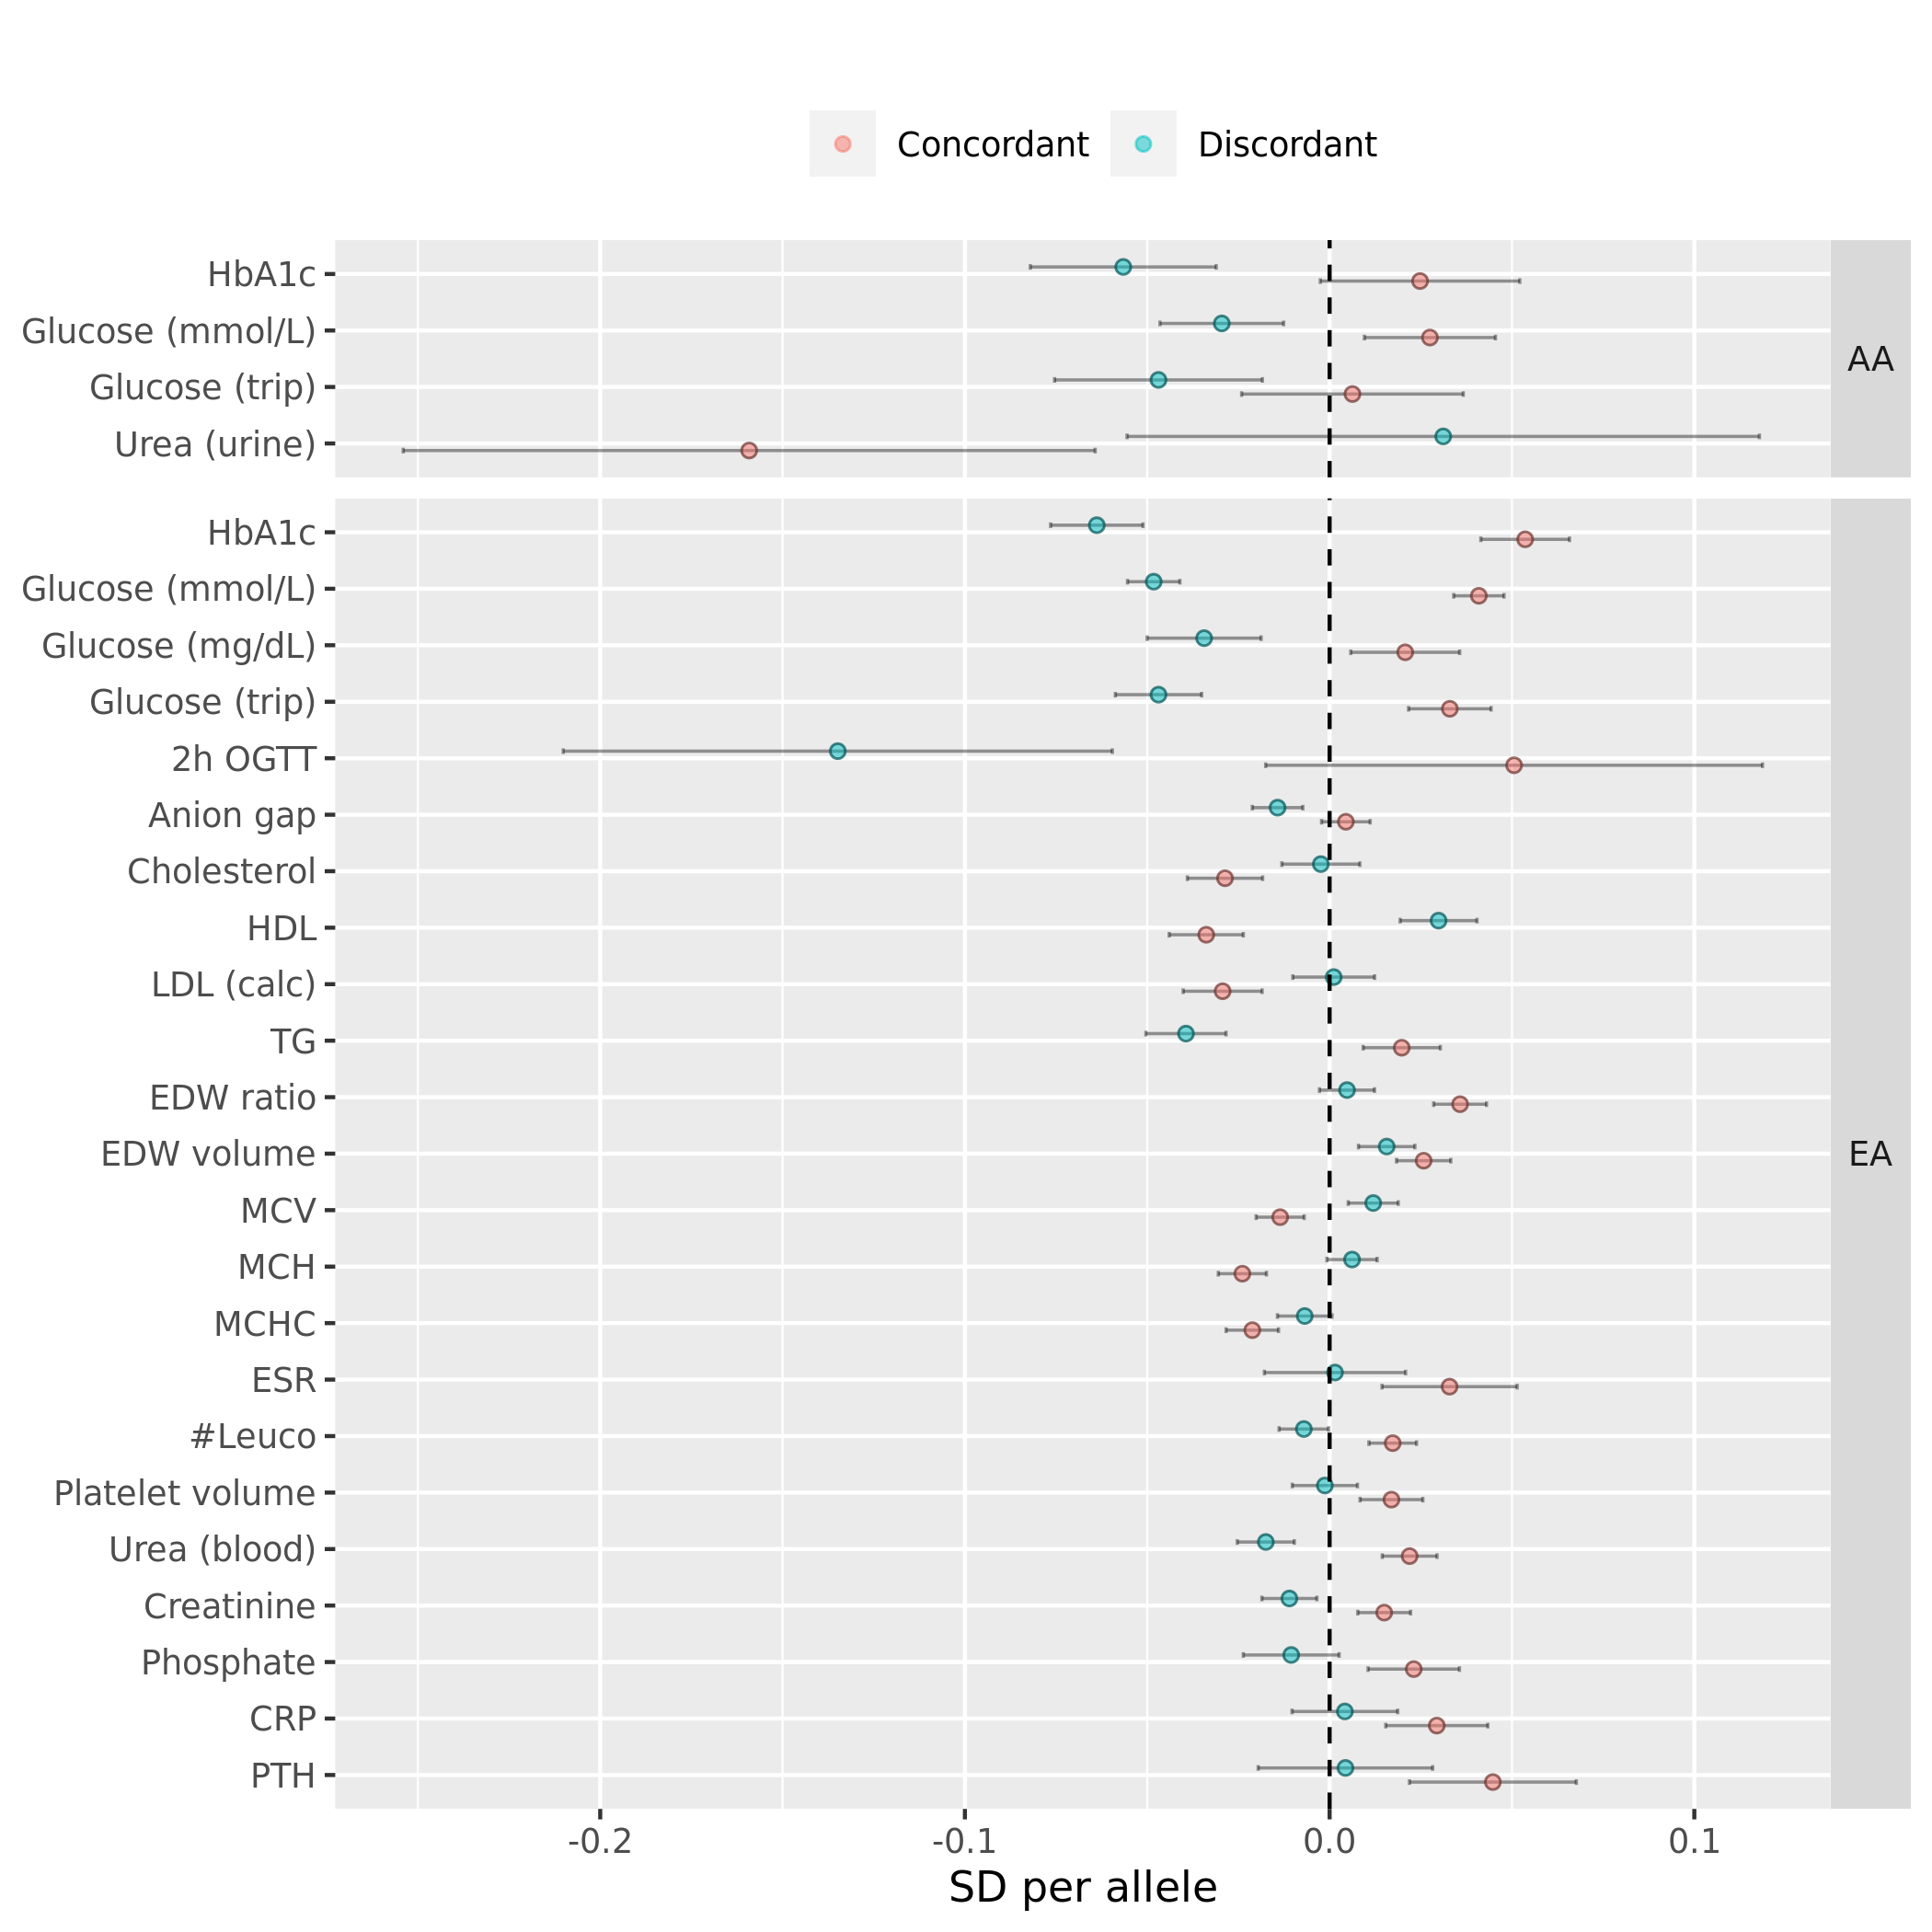
\includegraphics[width=7cm]{./plots/lw_biovu.png}
\caption{Concordant and discordant weight gain in BioVU}
\end{figure}
\end{frame}
\begin{frame}[label={sec:orgc4316e7}]{Mortality in UK Biobank - Concordant vs Discordant SNPs}
\begin{figure}[htbp]
\centering
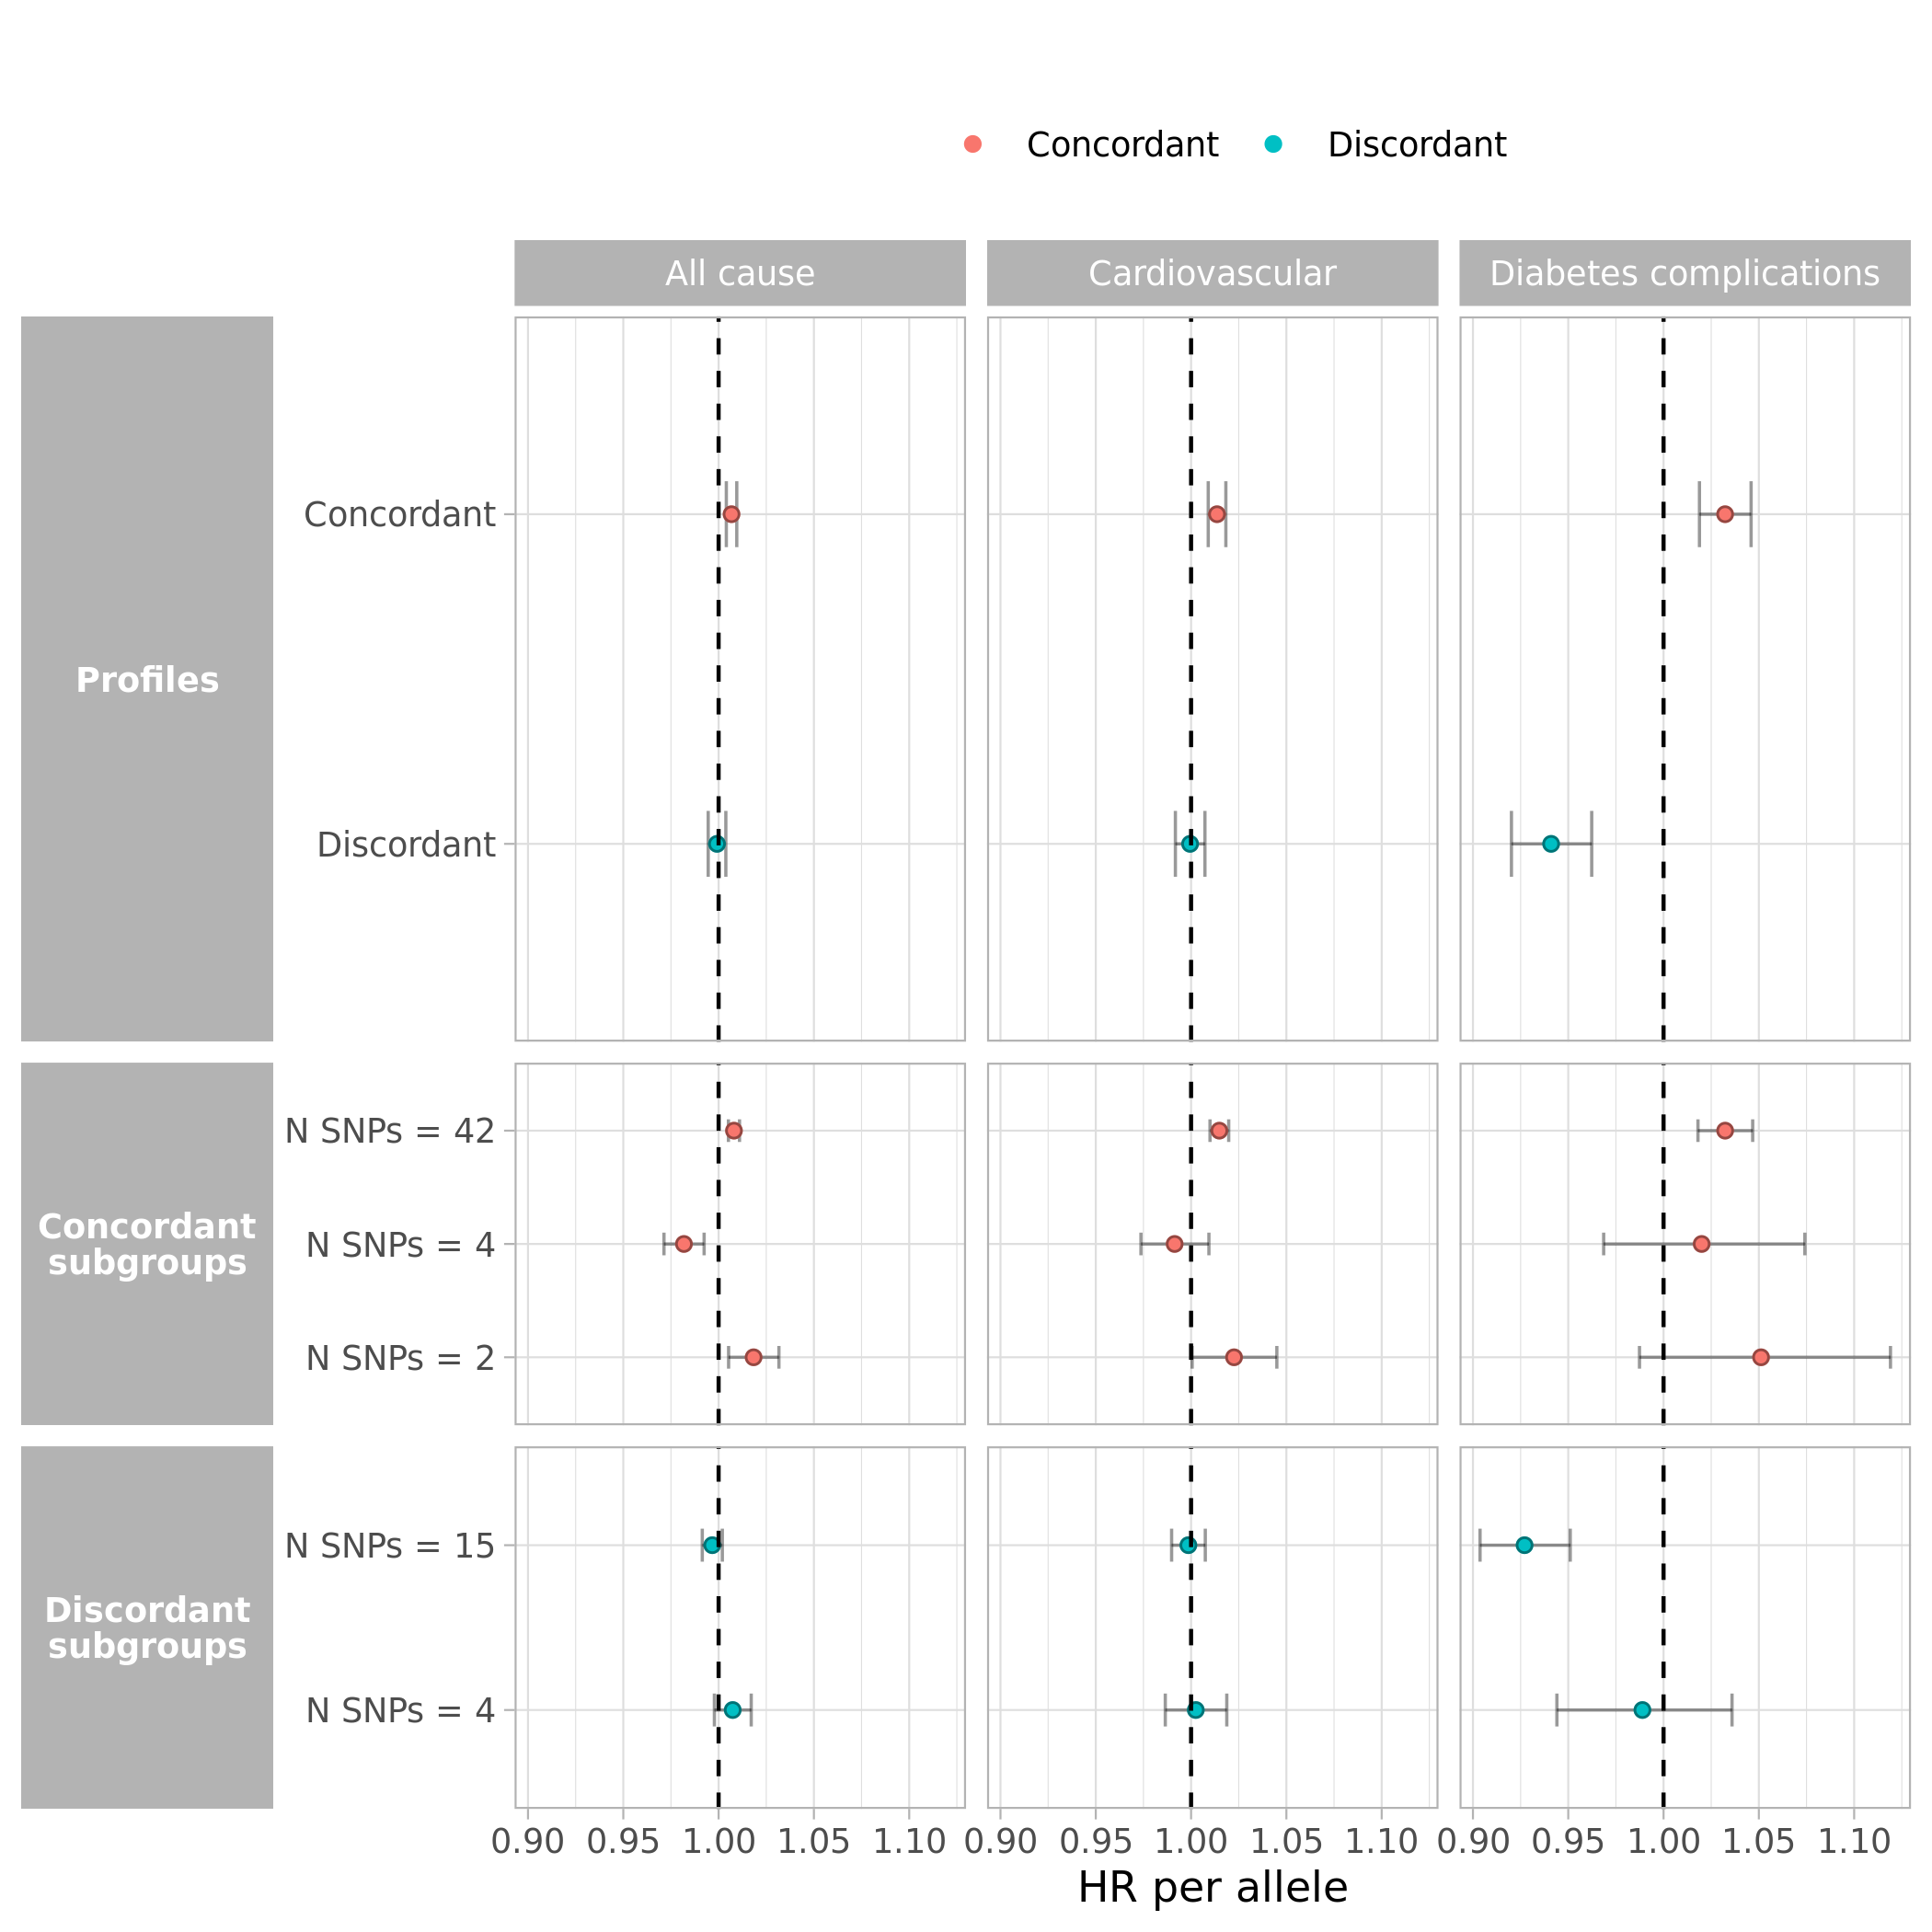
\includegraphics[width=7cm]{./plots/prs_surv.png}
\caption{Survival analysis of concordant and discordant PRS}
\end{figure}
\end{frame}
\begin{frame}[label={sec:org945cb9c}]{Mendelian Randomization}
\begin{center}
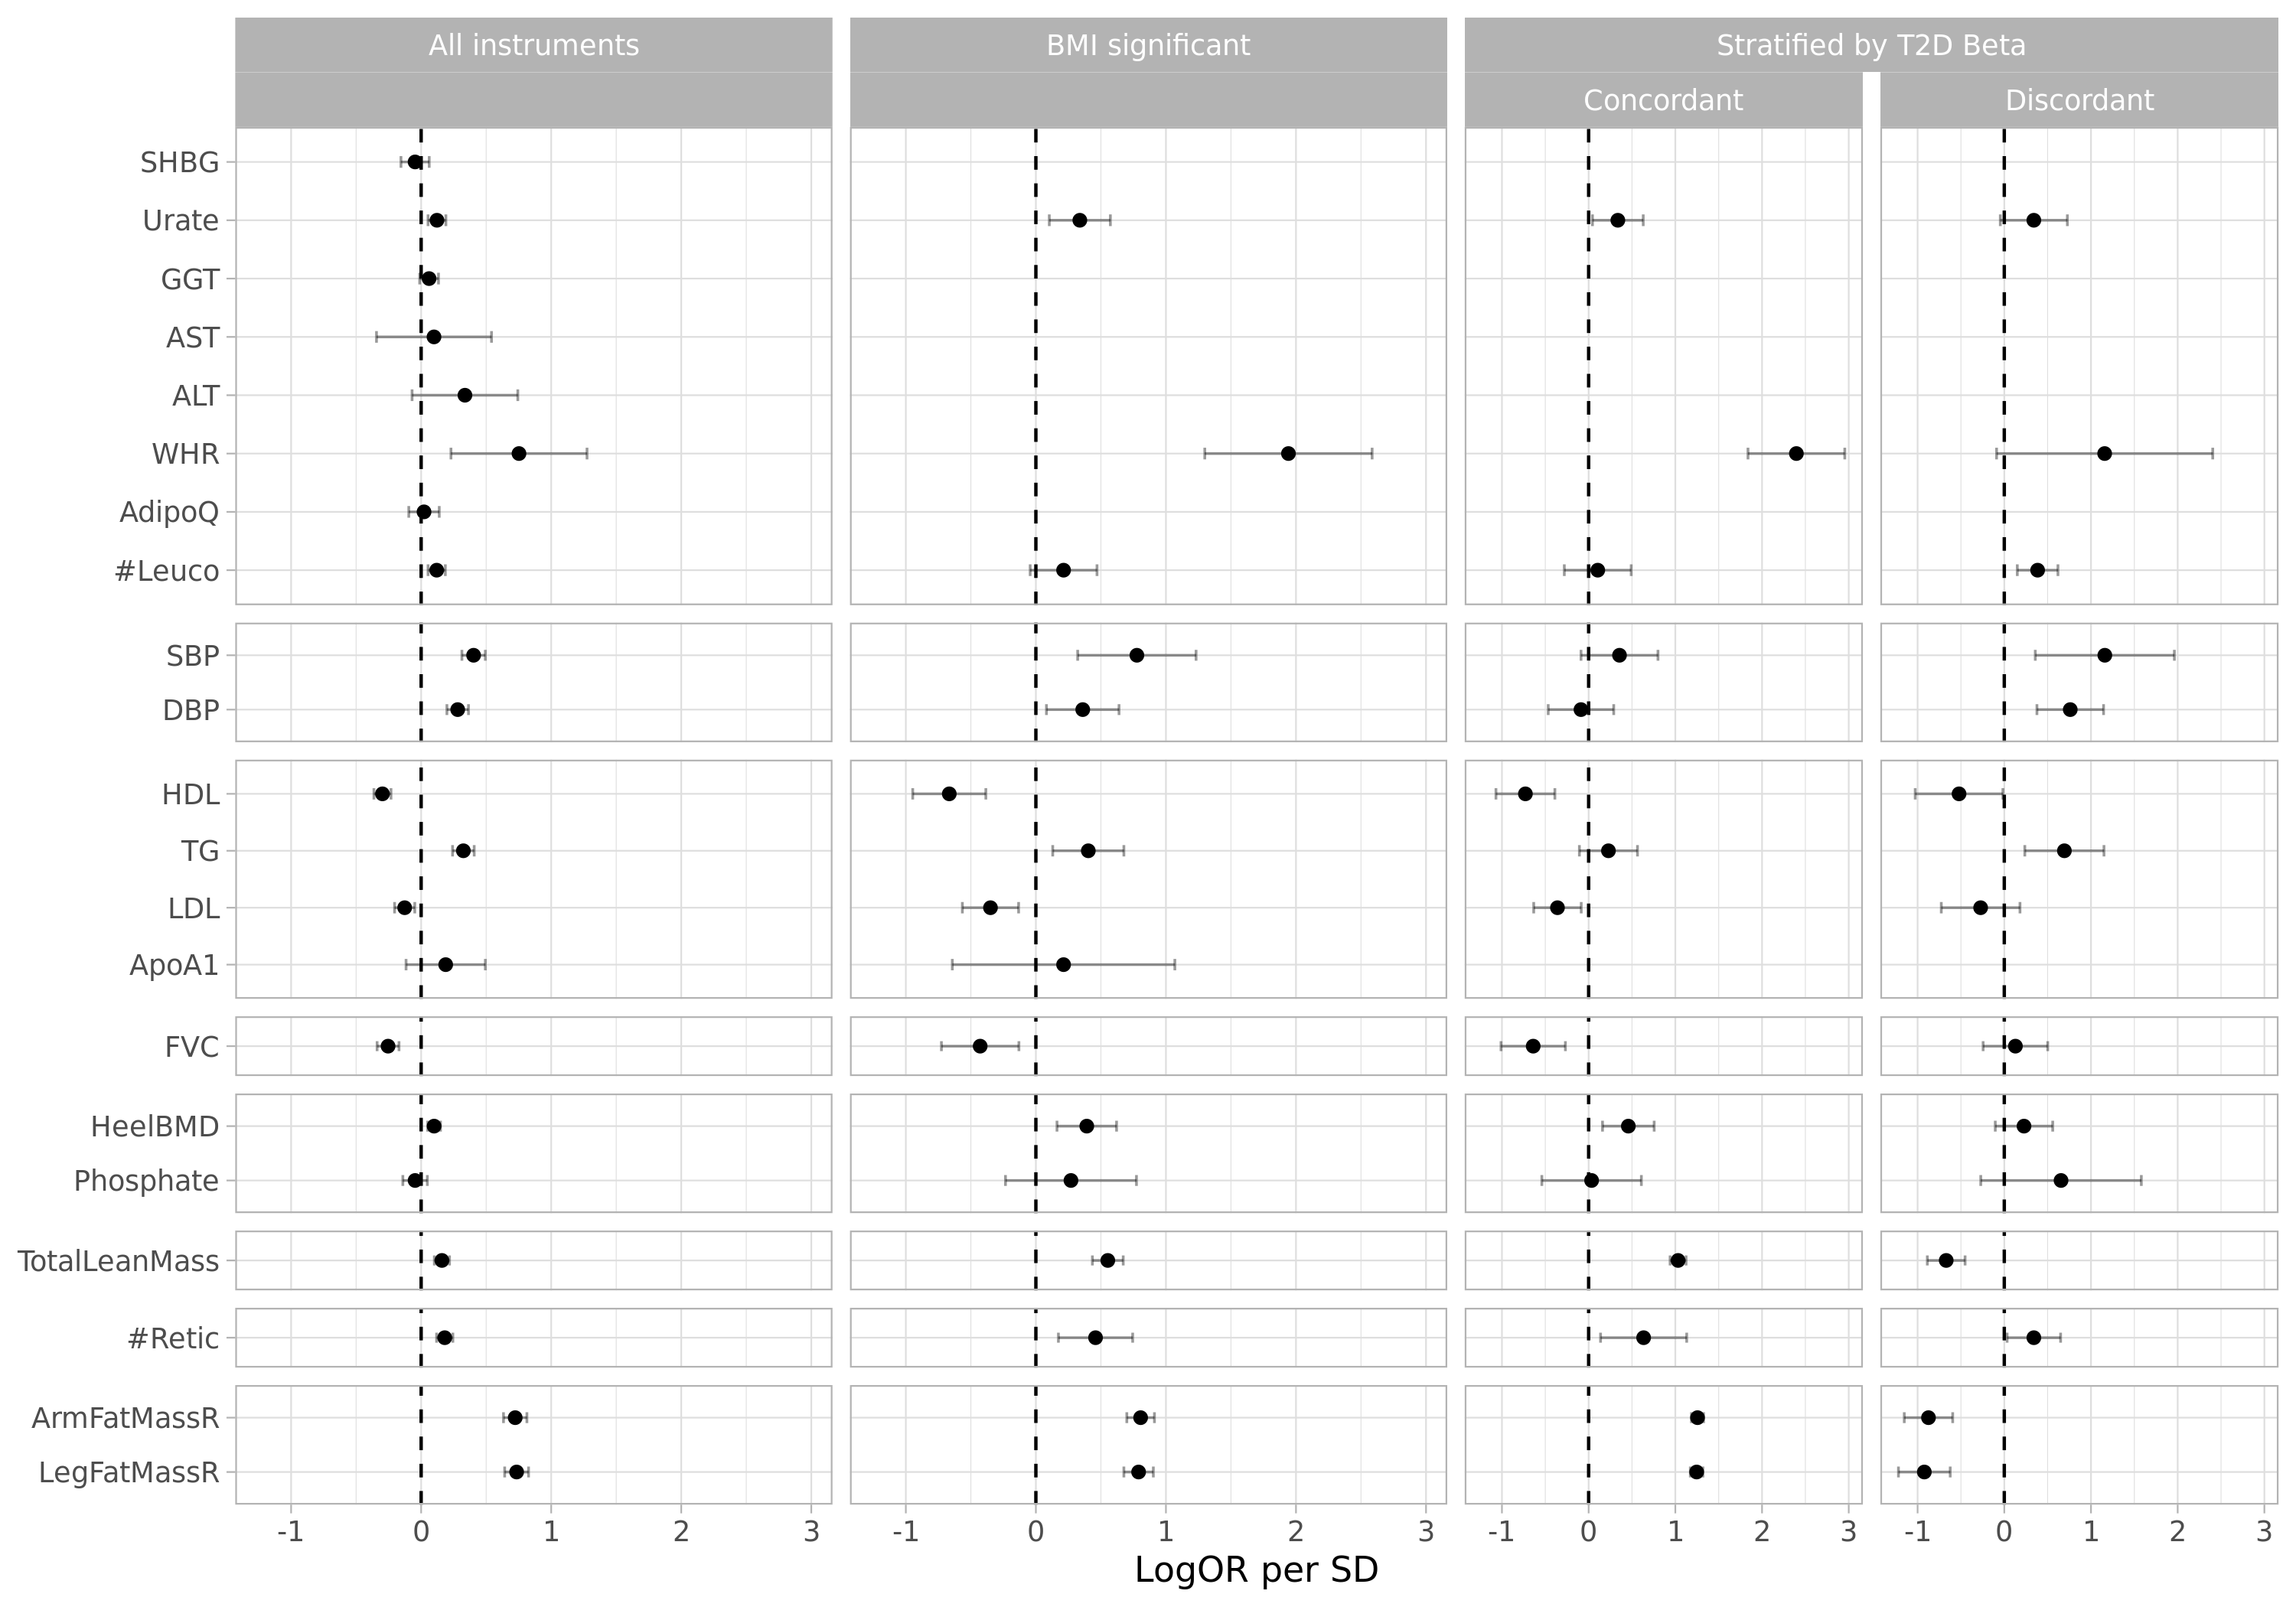
\includegraphics[width=7cm]{./plots/mr_res.png}
\end{center}
\end{frame}
\begin{frame}[label={sec:orge459bbf}]{Conclusions}
\begin{itemize}
\item Concordant and discordant SNPs differ mainly in:
\begin{itemize}
\item Liver enzymes - Central adiposity
\item Blood pressure
\item Lipids
\end{itemize}
\item And differ less strongly in:
\begin{itemize}
\item BMD
\item RBC counts
\item Overall adiposity
\end{itemize}
\item The two subgroups are not homogeneous
\item The causal pathways might differ
\end{itemize}
\end{frame}
\begin{frame}[label={sec:org1d93762}]{Strengths and limitations}
\begin{itemize}
\item Mechanisms uncoupling obesity from T2D
\item Agnostic approach
\item Reverse causality and confounding
\item Only EUR
\item Thresholds chosen affect:
\begin{itemize}
\item Genetic factors chosen
\item Clusters built
\end{itemize}
\item Smaller sets of instruments in stratified MR
\end{itemize}
\end{frame}
\begin{frame}[label={sec:org2ad2fda}]{Possible future applications}
\begin{itemize}
\item Other levels of the phenome
\item Random forest proximitry matrix to find more subtypes
\end{itemize}
\end{frame}
\end{document}
